\documentclass[a4paper,12pt,twoside,openright]{report}

\usepackage{graphicx}

\def\authorname{Jan S\"ondermann\xspace}
\def\authorcollege{Selwyn College\xspace}
\def\authoremail{jjes2@cam.ac.uk}
\def\dissertationtitle{Bayesian optimisation of approximateness in the trade-off between statistical and computational efficiency}
\def\wordcount{14279}

\usepackage{todonotes}
\usepackage{euscript}
\usepackage[export]{adjustbox}
\usepackage{subcaption}
\usepackage{chngpage}
\usepackage{calc}
\usepackage{epsfig,graphicx,parskip,setspace,tabularx,xspace} 
\usepackage{enumitem}
\usepackage{mathtools}
\usepackage{amsmath,amssymb}
\usepackage{algorithmicx}
\usepackage{algorithm}
\usepackage{algpseudocode}
\newcommand{\Break}{\State \textbf{break} }
\usepackage{color}
\usepackage{listings}
\usepackage{setspace}
%\lstset{breaklines=true, frame=single, numbers=left, basicstyle=\small\ttfamily}
\definecolor{Code}{rgb}{0,0,0}
\definecolor{Decorators}{rgb}{0.5,0.5,0.5}
\definecolor{Numbers}{rgb}{0.5,0,0}
\definecolor{MatchingBrackets}{rgb}{0.25,0.5,0.5}
\definecolor{Keywords}{rgb}{0,0,1}
\definecolor{self}{rgb}{0,0,0}
\definecolor{Strings}{rgb}{0,0.63,0}
\definecolor{Comments}{rgb}{0,0.63,1}
\definecolor{Backquotes}{rgb}{0,0,0}
\definecolor{Classname}{rgb}{0,0,0}
\definecolor{FunctionName}{rgb}{0,0,0}
\definecolor{Operators}{rgb}{0,0,0}
\definecolor{Background}{rgb}{0.98,0.98,0.98}

\lstset{
numbers=left,
numberstyle=\footnotesize,
numbersep=1em,
xleftmargin=1em,
framextopmargin=2em,
framexbottommargin=2em,
showspaces=false,
showtabs=false,
showstringspaces=false,
frame=l,
tabsize=4,
% Basic
basicstyle=\ttfamily\small\setstretch{1},
backgroundcolor=\color{Background},
language=Python,
% Comments
commentstyle=\color{Comments}\slshape,
% Strings
stringstyle=\color{Strings},
morecomment=[s][\color{Strings}]{"""}{"""},
morecomment=[s][\color{Strings}]{'''}{'''},
% keywords
morekeywords={import,from,class,def,for,while,if,is,in,elif,else,not,and,or,print,break,continue,return,True,False,None,access,as,,del,except,exec,finally,global,import,lambda,pass,print,raise,try,assert},
keywordstyle={\color{Keywords}\bfseries},
% additional keywords
morekeywords={[2]@invariant},
keywordstyle={[2]\color{Decorators}\slshape},
emph={self},
emphstyle={\color{self}\slshape},
%
}


\DeclareMathOperator*{\argmax}{arg\,max}


\begin{document}



\pagestyle{empty}
\singlespacing
% title page information
\begin{titlepage} 

\begin{center}
\noindent
\huge
\dissertationtitle \\
\vspace*{\stretch{1}}
\end{center}

\begin{center}
\noindent
\huge
\authorname \\
\Large
\authorcollege      \\[24pt]

\includegraphics{CUni3.eps}
\end{center}

\vspace{24pt} 

\begin{center}
\noindent
\large
{\it A dissertation submitted to the University of Cambridge \\ 
in partial fulfilment of the requirements for the degree of \\ 
Master of Philosophy in Advanced Computer Science} 
\vspace*{\stretch{1}}
\end{center}

\begin{center}
\noindent
University of Cambridge \\
Computer Laboratory     \\
William Gates Building  \\
15 JJ Thomson Avenue    \\
Cambridge CB3 0FD       \\
{\sc United Kingdom}    \\
\end{center}

\begin{center}
\noindent
Email: \authoremail \\
\end{center}

\begin{center}
\noindent
\today
\end{center}

\end{titlepage} 

\newpage
\vspace*{\fill}

\onehalfspacing
\newpage
{\Huge \bf Declaration}

\vspace{24pt} 

I \authorname of \authorcollege, being a candidate for the M.Phil in
Advanced Computer Science, hereby declare that this report and the
work described in it are my own work, unaided except as may be
specified below, and that the report does not contain material that
has already been used to any substantial extent for a comparable
purpose.

\vspace{24pt}
Total word count: \wordcount

\vspace{60pt}
\textbf{Signed}: 

\vspace{12pt}
\textbf{Date}:


\vfill

This dissertation is copyright \copyright 2010 \authorname. 
\\
All trademarks used in this dissertation are hereby acknowledged.



\newpage
\vspace*{\fill}

\singlespacing
\newpage
{\Huge \bf Abstract}
\vspace{24pt} 


% TODO write abstract
%Our project falls into the field of meta-machine learning that tries to use machine learning methods to improve the result of using these methods.


\newpage
\vspace*{\fill}


\newpage
{\Huge \bf Acknowledgements}
\vspace{24pt} 
\onehalfspacing

I would like to express my gratitude to my supervisor, Prof.\ Zoubin Ghahramani, for agreeing to supervise this dissertation after teaching me many of the concepts used in this project in his Machine Learning course.

I am very grateful to my co-supervisor, James Robert Lloyd, for proposing this topic and for his constant support and advice throughout the project.

My graduate study in Cambridge was made possible by a scholarship from the German Academic Foundation and a bursary from the the Computer Laboratory's Advanced Computer Science MPhil Scholarship scheme.


\singlespacing
\newpage
\vspace*{\fill}


\pagenumbering{roman}
\setcounter{page}{0}
\pagestyle{plain}
\tableofcontents
\listoffigures
\listoftables

\onehalfspacing


\chapter{Introduction}

\pagenumbering{arabic}
\setcounter{page}{1}

Before the advent of computers, statistical methods had to be simple enough to be calculable by hand which greatly limited the degree of complexity that these methods could reach \cite{tukey1977exploratory}. As computing power available to statisticians increased, many new methods were devised to make use of these new resources, in some cases exceeding the computational possibilities available.

Although machine learning is a diverse subject that combines influences from many different fields such as engineering, computer science, computational biology and physics, many of the recent advances have come from statistics or made use of statistical methods. As is true for mathematics more generally, considerations of runtime and complexity are usually not in the focus of attention in statistical research. This is in stark contrast to computer science, where the analysis of algorithmic complexity has been of great importance since the early beginnings of the field.

The cultural differences between computer science and statistics are revealed in the attitudes towards data that these fields exhibit: in computer science, data is seen as a workload to be completed with large amounts of data bringing with it the potential problem of uncontrollable growth of computational resources required. In statistics, however, the perception is that more data is always something desirable, allowing higher confidence in inferential results.

In recent years, the amount of scientific and commercial data available has increased rapidly, a phenomenon often labeled ``Big Data". As data science experts are facing the task of analysing these large datasets, controlling runtime has become increasingly important.

The current state of the field of machine learning requires skilled humans to make high level decisions on trade-offs between computational and statistical efficiency such as whether to use approximate inference methods or whether to use a simple method with lots of data rather than a complex method with a small amount of data. 

The necessary knowledge to make adequate decisions in these cases is often acquired through experience and requires an intuitive familiarity with the learning algorithms involved that can be hard to formalise and teach. As part of the current trend to automise all aspects of machine learning \cite{Lloyd2014-ABCD}, automating the process of finding an optimal balance in these trade-offs would make an important contribution to the field.

One way to add runtime considerations to statistical learning is to construct anytime algorithms \cite{conf/aaai/DeanB88}. Algorithms of this kind produce successively better results during the course of their execution. They can be terminated early, returning a result whose quality depends on the amount of time they were allowed to run for.

Another useful type of algorithm that requires an understanding of runtime are contract algorithms \cite{ZCCijcai99} that expect a dataset and a time budget as input and create an optimal model within the available time.

Given an algorithm with a number of ``approximation parameters" that control the degree of approximateness at which the algorithm runs, anytime and contract algorithms can be understood as optimisation problems. They find optima of the function mapping the approximation parameters to the time and predictive accuracy of the learning algorithms. In the process of optimisation, they have to take into account the additional runtime constraints that exist.

Classical optimisation methods may be ineffective in these cases as evaluating the function to be optimised can be an expensive computation. Further complicating this problem is the fact that the time required to evaluate the function can vary drastically depending on where it is evaluated: consider the case where the approximation parameter is the number of layers in a deep neural network. Increasing the number of layers will cause the inference to take more time. The optimisation routine has to consider this when optimising the function.

A natural solution to this problem is Bayesian optimisation as Bayesian optimisation methods make very efficient use of data when optimising a function.

Our first major contribution in this project is a model of how approximation parameters affect learning algorithm runtime and predictive accuracy. This model forms the foundation for the second major contribution of our system, a number of heuristics that use Bayesian optimisation methods to solve anytime and contract style problems as described above.

\begin{figure}
\centering
  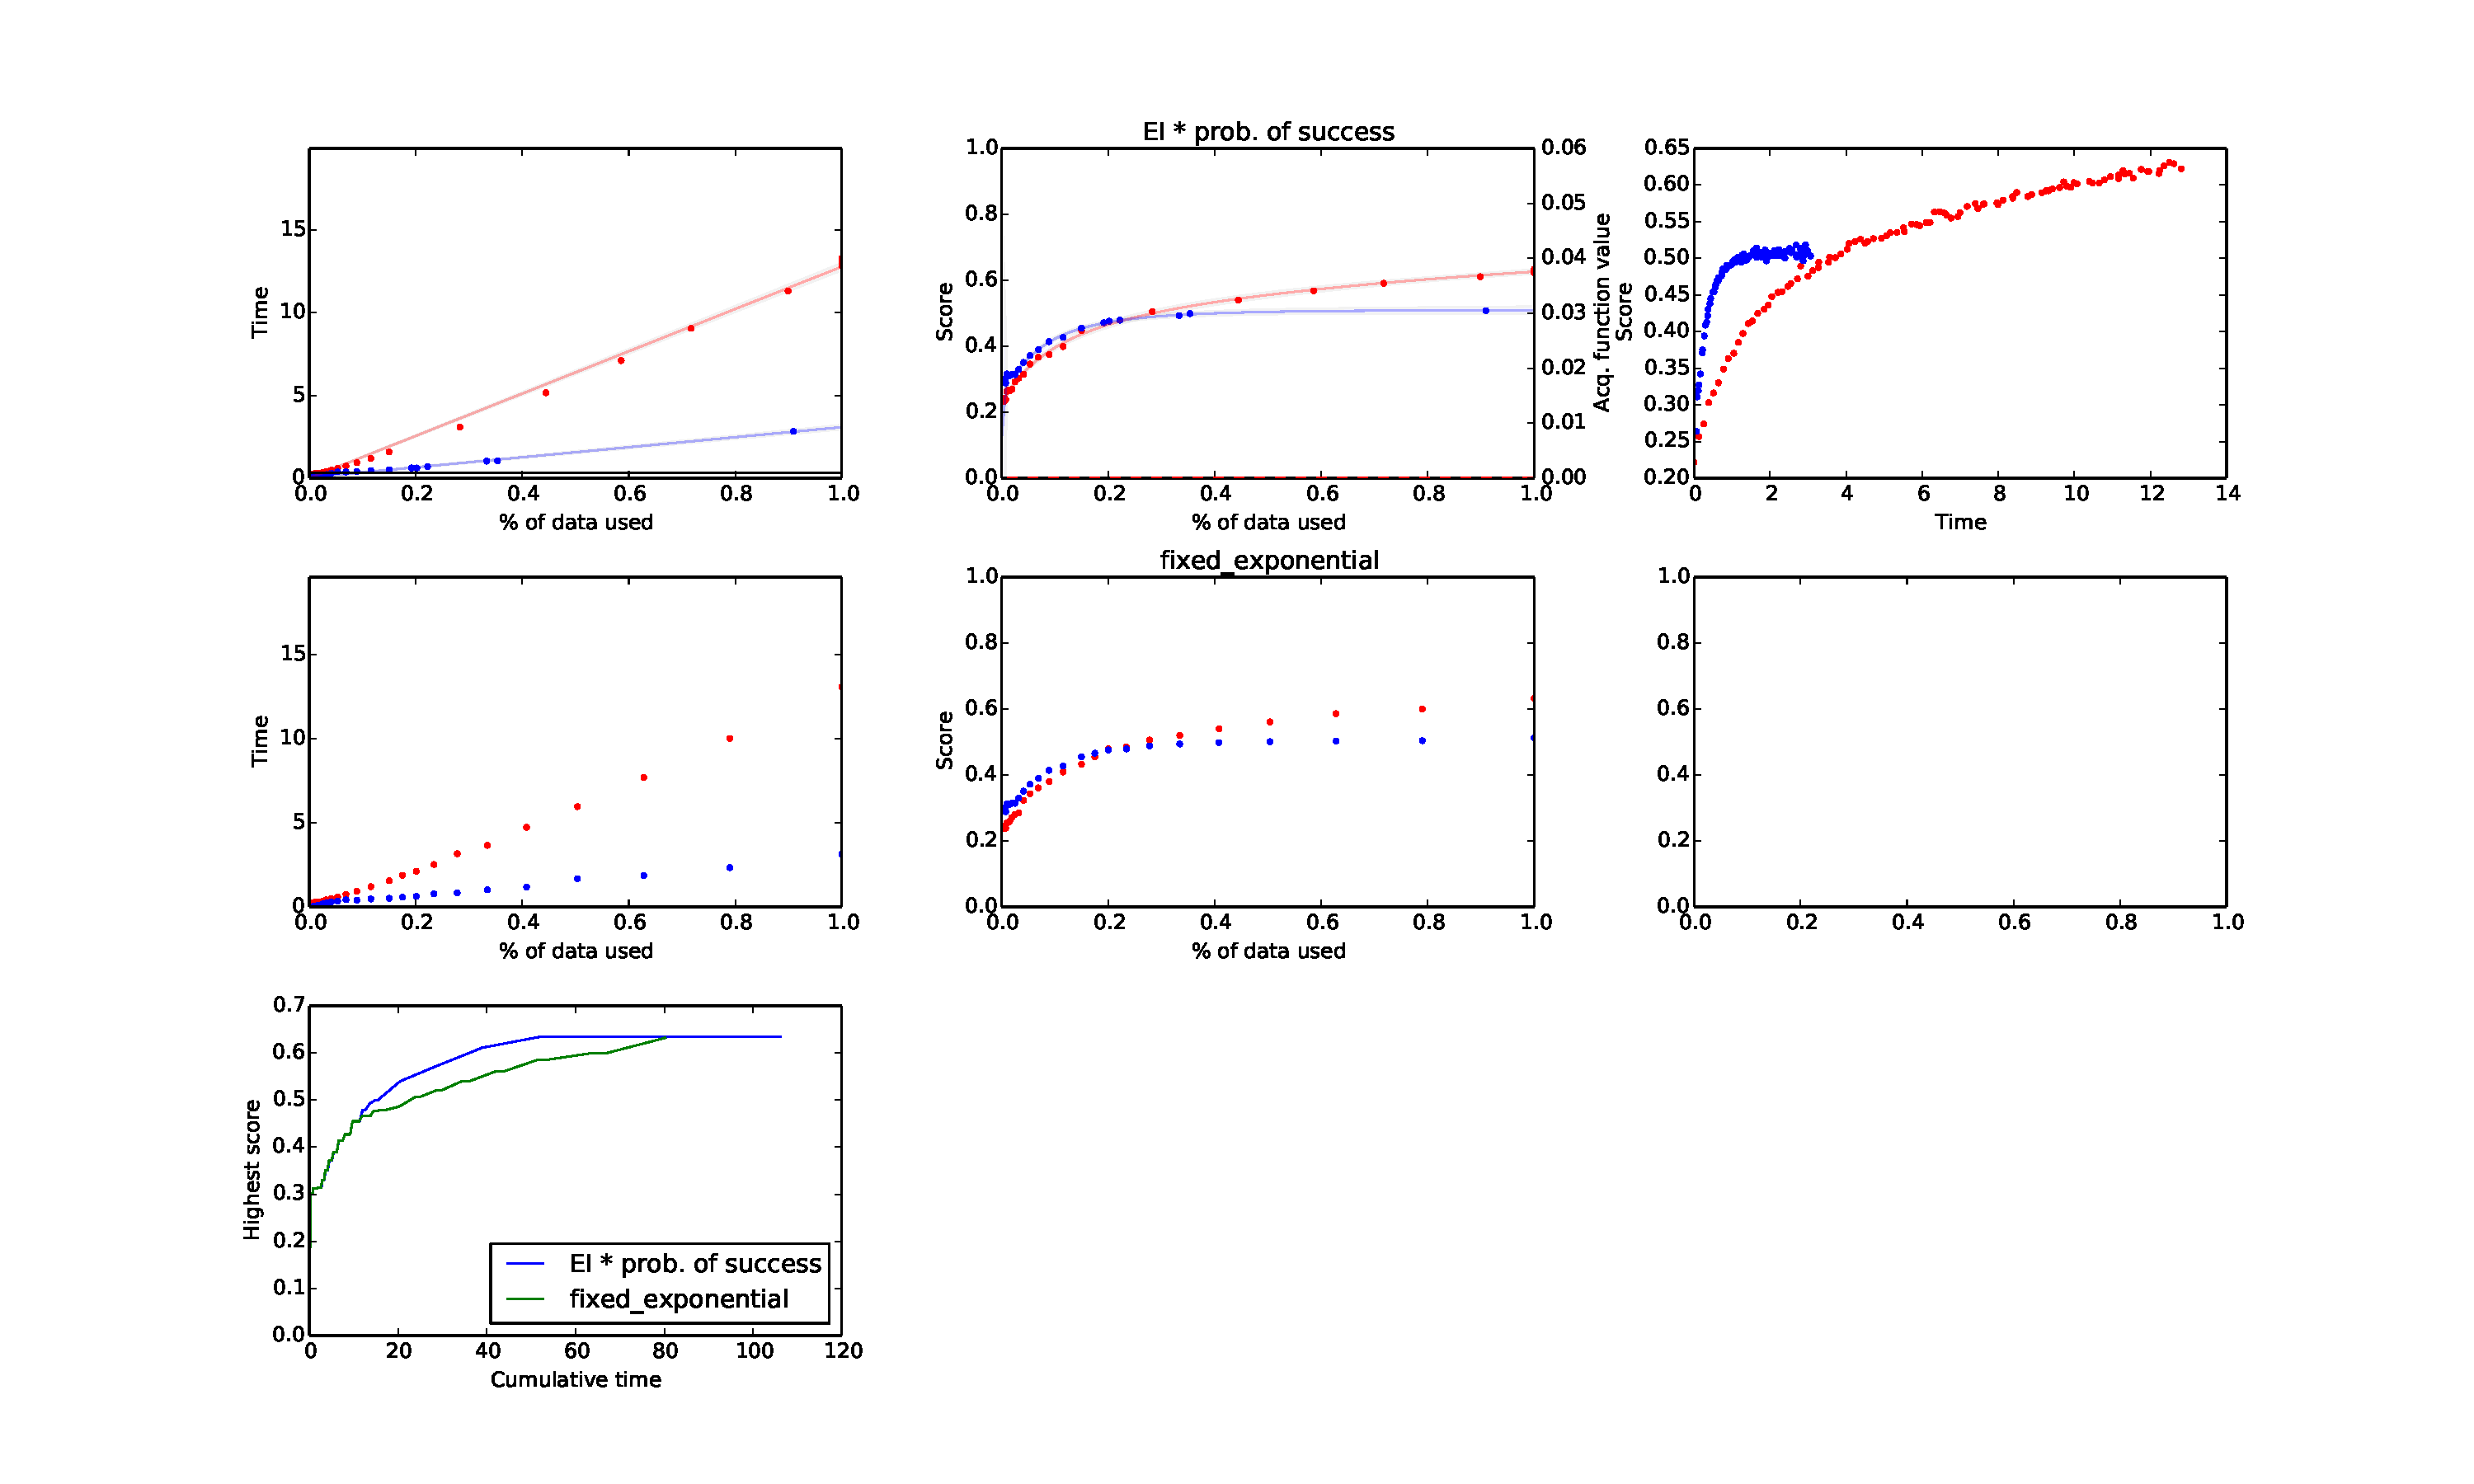
\includegraphics[trim=130 40 930 570,clip,width=\textwidth]{figures/anytime1.pdf}
  \caption{Comparing two heuristics}
  \label{anytime1}
\end{figure}


Figure \ref{anytime1} shows a plot that compares the performance of two anytime heuristics running in parallel. The $x$-axis shows the time in seconds that has elapsed since the start of the program while the $y$-axis shows the classification accuracy of the best model the heuristics have found. The ``\texttt{fixed\_exponential}" heuristic (shown in green) is a naive implementation used as a baseline that simply uses a fixed sequence of values for the approximation parameter. The ``\texttt{EI * prob.\ of success}" heuristic (shown in blue) is a more advanced heuristic which is explained in detail below. 

Both heuristics spend about 10 seconds in a burn-in phase during which they build the same models. After this burn-in ends, the blue heuristic immediately starts producing better models than the green heuristic and plateaus at the maximum value about 50 seconds after learning starts. To reach the same classification accuracy, the naive heuristic needs about 80 seconds.

Although both heuristics reach the same final accuracy eventually, if we terminate them after 30 seconds, the best model found by the ``\texttt{EI * prob of success}" heuristic is substantially better than the one found by the naive heuristic at this point, which makes it a better anytime algorithm. 

Besides this anytime heuristic, we also describe a contract heuristic that constructs models in a given time budget.


The remainder of this report is structured as follows:
\begin{itemize}
	\item The \textbf{Background} chapter introduces the theoretical background that this project is built on. It also lists the third-party libraries that were used during development
	\item The \textbf{Related Work} chapter summarises the current state of research on the problems we are trying to make a contribution towards solving
	\item The \textbf{Modelling Learning Time and Score} chapter explains how we model the performance of the learning algorithms using Gaussian processes
	\item The \textbf{Scheduling} chapter describes the architecture of the software we have written. It also lists and explains the heuristics we developed
	\item The \textbf{Evaluation} chapter examines the system we have built by describing and evaluating its results. It also lists challenges we faced and limitations of our current implementation
	\item The \textbf{Conclusion and future work} chapter recapitulates our results by returning to the broader context lined out in this introduction and lists possible ways of extending the existing system
\end{itemize}


\chapter{Background}
\textit{This chapter describes the background assumed in the remainder of the document. We give a brief explanation of general machine learning principles together with a summary of the algorithms used in this project, including Gaussian processes which form the basis of the Modelling chapter. We then describe Bayesian optimisation which is the method underlying the ideas described in the Schedulers chapter, and briefly mention third-party software we used to build our system.}


\section{Key Concepts}
\begin{figure}
\centering
  \includegraphics[width=\textwidth]{figures/ml.pdf}
  \caption{The general process of learning from data with training data}
  \label{mlstructure}
\end{figure}

Our project falls into the field of meta-machine learning. We use machine learning algorithms to learn and predict the performance of other machine learning algorithms. This necessitates a brief overview of machine learning principles: Figure \ref{mlstructure} shows the general structure of learning from data: the learning algorithm expects some training data together with a set of hyperparameters and outputs a function $\hat{f}$, usually called the model, that models the true function $f$ underlying the data. This function is subsequently used to make predictions on unseen data.

Of particular relevance to our project is the second input to the learning algorithm, its hyperparameters. These hyperparameters control the behaviour of the learning algorithm and influence the quality of the model which makes selecting appropriate hyperparameters crucial.


\subsection{Approximation Parameters}
By ``approximation parameters", we denote parameters to machine learning algorithms that influence the trade-off between statistical and computational efficiency, letting us vary the degree of approximateness at which the algorithm runs. Changing an approximation parameters should either decrease the runtime at the cost of classification accuracy or improve accuracy while making the process of creating the model slower. 

The approximation parameter that we put most of our focus on in this project is the proportion of the available data. Other approximation parameters are hyperparameters to the machine learning algorithms such as the number of decision trees in a random forest.

Note that not all hyperparameters are approximation parameters. Some hyperparameters influence performance without changing the runtime such as the length-scales of Gaussian process kernels, explained in depth in the Gaussian process section of this chapter\footnote{Many machine learning packages include parameters such as the number of threads used for learning in their APIs. These are parameters that influence runtime but not performance. They are, however, particular to the implementation and not part of the algorithm.}.

\subsection{Scheduling}
As mentioned in the introduction, the problem we try to solve in this project is an optimisation problem with the additional component of runtime constraints. A solution to this problem consists in devising strategies to decide on a sequence of evaluations of the function to be optimised, such that we find an optimum within these constraints. 

We use the term ``scheduler" to denote heuristics that select such a sequence. Schedulers allocate the time available to building models during optimisation. We will use the terms ``scheduler" and ``heuristic" interchangeably in the remainder of this document.

\subsection{Time, Score and Performance}
The learning process can be measured in two ways: the time it takes to create a model and the quality of the predictions the model makes. We denote this predictive strength by ``score" and call both the time and score together the learning algorithm's performance.

\section{Machine Learning Algorithms}
\subsection{Logistic Regression and Random Forests}
This subsection introduces the two machine learning algorithms that we focus on in the evaluation of our system, logistic regression and random forests. These two algorithms are among the most common machine learning algorithm and are frequently used in real world applications.

\subsubsection{Logistic regression}

Logistic regression is a variant of linear regression, a widely used machine learning algorithm \cite{1958, Murphy:2012:MLP:2380985}. In linear regression, the model $\hat{f}$ has the form
\begin{equation}
\hat{f}(\mathbf{x}) = \mathbf{w}_0 + \sum_{i=1}^n \mathbf{w}_i \mathbf{x}_i
\end{equation}

where the vector $\mathbf{w}$ is the model parameter vector and $n$ is the number of features. Fitting the model to data is achieved by adapting these parameters.

Linear regression is used for regression problems, where the values to be predicted are continuous. The datasets we consider in this report belong to a different type, where the required output is a label taken from a finite set of classes.

In the simplest case of such classification problems, binary classification, each sample belongs to one of two classes. To obtain appropriate outputs, we wrap the computation of $\hat{f}$ in a function that forces all values into the range from 0 to 1. A commonly used function with this property is the sigmoid function $\sigma(x) = \frac{1}{1+e^x}$. We assign the classes to 0 and 1, such that values for $\hat{f}$ close to 1 are to be interpreted to mean that the sample is likely to be of class 1.

In the multiclass case with $c$ classes, the machine learning library used in this project employs a technique called one-vs-all. It constructs $c$ functions $\hat{f}^{(c)}$. Each function performs a binary classification between the class with index $c$ and all other classes, such that for samples likely to belong to class with index $c$, $\hat{f}^{(c)}$ has values close to 1. $\hat{f}$ is computed by selecting the class for which $\hat{f}^{(c)}$ is largest.

\subsubsection{Random forests}
Random forests, introduced in \cite{rndforests}, is an algorithm that extends the idea of decision trees, a simple learning method. Decision trees are grown by repeatedly splitting the feature space into rectangular regions such that the proportion of samples of the same class in a region is maximised \cite{james2014introduction}. 

Individual decision trees alone can not compete with the predictive performance of other common algorithms \cite{hastie01statisticallearning}. In particular they suffer from high variance, meaning that multiple trees created using the same dataset often make substantially different predictions. An initial solution to this, proposed in \cite{bagging}, is Bagging, a technique that creates a number of new training sets by drawing samples from the original dataset. The trees are then fitted to these new training sets. To make a prediction, the predictions of all trees are averaged over.

Random forests improve the results obtained by bagging through decorrelating the trees. This is achieved by only considering a subset of features from the full set of features at each training step and prevents the trees from choosing the same features in the same order. By combining and averaging over a set of decision trees as described, random forests achieves a performance that makes it a popular choice in machine learning.

The number of trees is a possible approximation parameter to random forests. Another hyperparameter that is also an approximation parameter, is the minimum number of samples that must be contained in each region of the feature space for the trees in the forest.

\subsection{Gaussian Processes}
Gaussian processes are a machine learning method that generalises Gaussian distributions from single and multivariate distributions to distributions over functions \cite{Rasmussen:2005:GPM:1162254}. Unlike methods such as logistic regression that learn by updating a set of model parameters, Gaussian processes place a prior distribution directly over the function $\hat{f}$ \cite{Murphy:2012:MLP:2380985}. For this reason, they belong to a family of learning algorithms called nonparametric algorithms. To learn, the prior of a Gaussian process is updated to a posterior based on the training data using Bayes' theorem.

If we think of functions as infinitely sized vectors indexed by the domain of the function, Gaussian processes can be understood as a generalisation of the multivariate Gaussian distribution to a distribution over infinitely many variables. Formally, a multivariate Gaussian distribution $\mathcal{N}(\mu, \Sigma)$ is specified by a mean vector $\mu$ and a covariance matrix $\Sigma$. Equivalently, a Gaussian process $\EuScript{G}\EuScript{P}(m, \kappa)$ is specified by a mean function $m(x)$ and a covariance function\footnote{if we think of infinite vectors as single valued functions, infinitely large matrices can be seen as functions with two arguments.} $\kappa(x, x')$. It is common for the mean function to be a constant function with $\mu(x) = 0$ since the mean can be included in the covariance function. Covariance functions are also commonly called kernels. We will use the two terms interchangeably.

If we draw a function $f \thicksim \EuScript{G}\EuScript{P}(m, \kappa)$ from a Gaussian process, every finite set of inputs to the function $\mathbf{x} = (x_1, \cdots, x_n)$ span a multivariate Gaussian distributed vector $\mathbf{f} = (f(x_1), \cdots, f(x_n)) \thicksim \mathcal{N}(\mu,K)$ with $\mu = (m(x_1), \cdots, m(x_n))$ and $K_{ij} = \kappa(x_i, x_j)$.

To encode prior assumptions about the nature of the functions to be modelled by a Gaussian process, one chooses a covariance function that expresses these assumptions by assigning appropriate covariances. There is a set of commonly used covariance functions that Gaussian process libraries usually implement. In the remainder of this section, we explain how prior information is reflected in the covariance functions by describing two such functions. We will return to this topic in the Modelling chapter when we describe the implementation of a custom covariance function. 

\subsubsection{The squared exponential kernel}
The squared exponential kernel is often chosen as a default kernel in Gaussian process modelling and, as such, very widely used. This kernel defines 

\begin{equation}
	\kappa(x, x') = \text{exp}(-\frac{(x-x')^2}{2\ell^2})
\end{equation}

with $\ell$ being the characteristic length-scale of the kernel. Figure \ref{sekernel} shows how the value of the squared exponential kernel changes as $x'$ moves away from $x$. 

The value of $\kappa(x, x')$ can be interpreted as the degree of similarity between $f(x)$ and $f(x')$ with larger values of $\kappa$ indicating higher similarity. This means that the squared exponential kernel expresses the prior that the functions to be modelled by the Gaussian process will be smooth, since $\kappa(x, x')$ is larger for closer values for $x$ and $x'$. Precisely how smooth they will be is determined by the length-scale $\ell$. This is a hyperparameter to the squared exponential kernel. These hyperparameters allow separating general prior assumptions, such as the assumption that the functions to be modelled will be smooth, from specific degrees of ``smoothness". Figure \ref{sekernel_ls} shows how changing the value of $\ell$ influences the shape of the kernel function.

\begin{figure}[t]
\centering
\begin{subfigure}{.45\textwidth}
\centering
  \includegraphics[trim=140 240 125 260,clip,frame,width=\textwidth]{figures/se_kernel.pdf}
  \caption{The squared exponential kernel with $x$ fixed in the center and $x'$ varying}
  \label{sekernel}
\end{subfigure}
\begin{subfigure}{.45\textwidth}
\centering
  \includegraphics[trim=140 240 125 260,clip,frame,width=\textwidth]{figures/se_kernel_different_ls.pdf}
  \caption{Three different values for $\ell$ for the squared exponential kernel with $x$ fixed in the center and $x'$ varying}
  \label{sekernel_ls}
\end{subfigure}
\caption{Plots of the squared exponential covariance function}
\label{se_covfunc}
\end{figure}

Figure \ref{sekernel_draws} shows five functions drawn from a Gaussian process with a squared exponential kernel and $\ell = 1$. Note how although the functions take different values, they share the same degree of smoothness. Figure \ref{sekernel_draws_different_ls} shows the effect that varying $\ell$ has on the functions by depicting three functions drawn from three different Gaussian processes that have squared exponential covariance functions with different length-scales. For smaller values, the functions become more rugged while increasing $\ell$ makes the function even smoother.

\begin{figure}[h]
\centering
\begin{subfigure}{.45\textwidth}
\centering
  \includegraphics[trim=120 240 100 240,clip,width=\textwidth]{figures/se_kernel_draws.pdf}
  \caption{Five draws from a Gaussian process with a squared exponential kernel}
  \label{sekernel_draws}
\end{subfigure}
\begin{subfigure}{.45\textwidth}
\centering
  \includegraphics[trim=120 250 100 220,clip,width=\textwidth]{figures/se_kernel_draws_different_ls.pdf}
  \caption{Functions drawn from Gaussian processes with squared exponential kernels that have different length-scales}
  \label{sekernel_draws_different_ls}
\end{subfigure}
\caption{Draws from Gaussian processes}
\label{se_gp_draws}
\end{figure}

The squared exponential kernel is an example of a class of kernels called \emph{stationary kernels}. These kernels  have the property that their value does not change if $x$ and $x'$ are shifted by the same amount. Formally, for stationary kernels, $\kappa(x, x') = \kappa(\tau + x, \tau + x')$. This means that the degree of smoothness that functions drawn from a Gaussian process with a squared exponential kernel exhibit, is constant over the entire domain of the function.


\subsubsection{The linear kernel}
The linear kernel is defined as $\kappa(x, x') = (x-c)(x'-c)$ with $c$ determining the $x$-coordinate of the point that all the functions in the posterior pass through \cite{duvenaudthesis}. The linear kernel is an example of a kernel that is not stationary as it encodes the prior information of global, linear change in the functions it models.


\subsubsection{Combining kernels}
Although there is a substantial number of these common kernels, their number is still finite. To express more complex priors, it is therefore necessary to either combine existing kernels or write entirely new ones. One way to combine two existing kernels is to add them together. Figure \ref{sum_of_lin_and_se} shows functions drawn from a Gaussian process that has as its kernel the sum of a squared exponential and a linear kernel. It combines a linear component with the noisiness of the squared exponential kernel.

\begin{figure}[h!]
\centering
\begin{subfigure}{.45\textwidth}
\centering
  \includegraphics[trim=80 210 70 170,clip,width=\textwidth]{figures/sum_of_lin_and_se.pdf}
  \caption{Adding a linear kernel to a squared exponential kernel}
  \label{sum_of_lin_and_se}
\end{subfigure}
\begin{subfigure}{.45\textwidth}
\centering
  \includegraphics[trim=80 210 70 205,clip,width=\textwidth]{figures/prod_of_lin_and_lin.pdf}
  \caption{Multiplying two linear kernels}
  \label{prod_of_lin_and_lin}
\end{subfigure}
\caption{Combining kernels}
\label{combining_kernels}
\end{figure}

Another way to combine kernels is multiplication. Figure \ref{prod_of_lin_and_lin} shows the result of multiplying to linear kernels together, which results in a kernel that produces quadratic functions.



\subsubsection{Marginal Likelihood}
The marginal likelihood of some data $y$ for a Gaussian process input data $\mathcal{D}$ and hyperparameters $\theta$ is obtained by integrating over the functions $f$ that the Gaussian process defines a distribution over. Formally:
\begin{equation}
p(\mathbf{y}|\mathcal{D}, \theta) = \int p(\mathbf{y}|f, \mathcal{D}, \theta)p(f|\mathcal{D}, \theta) df
\end{equation}

Comparing the marginal likelihood of two models allows us to choose the one that better fits the data.


\section{Bayesian Optimisation}
Bayesian optimisation is a method to solve the optimisation problem of having to find an $x$ that maximises\footnote{We will consider maximisation only in this section as minimising $f$ is equivalent to maximising $-f$} $f(x)$ for a given function $f$, formally: 

\begin{equation}
\argmax_x f(x)
\end{equation}

Bayesian optimisation is based on the idea of placing a prior over the function $f$. After evaluating $f$ and obtaining a new data point, the model of $f$ is updated and used to decide where to evaluate the function next.

Since Gaussian processes are precisely such priors over functions, they are well suited to be used to construct models for Bayesian optimisation. By selecting an appropriate kernel, as described in the previous section, one can express existing prior knowledge over the function to be optimised which is crucial in ensuring that the Bayesian optimiser makes adequate choices when deciding the sequence of function evaluations.

Unlike other optimisation methods like gradient descent that only use information local to the function at the last evaluation, Bayesian optimisation considers all the available data when deciding where to evaluate the function next. This means that Bayesian optimisation often finds an optimum in fewer steps than other methods. This, however, comes at the cost of requiring more computational resources to make the decision of where to next evaluate the function \cite{PracticalBayesianOptimization}.

These properties make Bayesian optimisation especially well suited for cases like ours where evaluating $f$ is potentially very costly and the number of function evaluation should be minimised. In addition, Bayesian optimisation has been shown to be successful at optimising hyperparameters of machine learning algorithms \cite{PracticalBayesianOptimization}. This is a problem that shares many similarities with the one our project addresses.

To make a decision about where to evaluate $f$, Bayesian optimisation constructs an acquisition function $a$ using its model of $f$. This acquisition function is used as a proxy for $f$ by calculating $x_{\text{next}} = \argmax_x a(x)$.

There are several standard ways to construct the acquisition function $a$ when using Bayesian optimisation. In the remainder of this section, we explain two common strategies, maximising the probability of improvement and maximising the expected improvement. In the Scheduling chapter, we describe custom acquisition functions that take runtime constraints into account when deciding where to evaluate $f$.

Figure \ref{bayesianopti} shows an example of using Bayesian optimisation to find the maximum of a function. The topmost plot shows the function $f$ as a dashed, blue line. This is the true, underlying function to which we only have access through individual evaluations. This function has been evaluated seven times and the Gaussian process model that models the function using the information gained in these evaluations is drawn with the mean shown as a red line and twice the standard deviation shown in grey. This is the information that is available to the acquisition function $a$.

\begin{figure}[p]
\centering
  \includegraphics[trim=60 120 60 120,clip,width=\textwidth]{figures/bayesian_opti.pdf}
  \caption{Two different acquisition functions for Bayesian optimisation. In the top plot, the blue dashed line is the underlying function, the red line is the mean of our model and the shaded area is twice the standard deviation}
  \label{bayesianopti}
\end{figure}
The second plot shows the acquisition function that computes the probability of improvement. This acquisition function is based on the strategy of finding the point most likely to yield an improvement over the current maximum $y_{\text{max}}$. It is calculated as
\begin{align}
a_{PI}(x) &= P(y \geq y_{\text{max}}) \text{\ with\ } y \thicksim \mathcal{N}(\mu(x),\sigma^2(x))\label{eq:pi_equation}\\
&=\Phi(\frac{\mu(x) - y_{\text{max}}}{\sigma(x)})
\end{align}
where $\mu$ and $\sigma$ are the mean and variance of the Gaussian process model.

A superior strategy to decide which point to evaluate next is to maximise the expected improvement which is calculated as follows:

\begin{align}
a_{EI}(x) &= \mathbb{E}(\text{max}\{y - y_{\text{max}}, 0\}) \text{\ with\ } y \thicksim \mathcal{N}(\mu(x),\sigma^2(x))\\
&= \mathbb{E}(\begin{cases}
        y-y_{\text{max}} \text{\ \ if\ \ } y \geq y_{\text{max}}
        \\
        0 \text{\ \ \ \ \ \ \ \ \ \ \ \ otherwise}
        \end{cases})\\
&= \int_{y_{\text{max}}}^\infty (y-y_{\text{max}})p(y)dy\\
&= \int_{y_{\text{max}}}^\infty y\cdot p(y)dy-y_{\text{max}}\int_{y_{\text{max}}}^\infty p(y)dy\\
&= \sigma(x)\phi(\frac{y_{\text{max}}-\mu(x)}{\sigma(x)}) + \mu(x)\Phi(\frac{\mu(x) - y_{\text{max}}}{\sigma(x)}) \\
&\quad - y_{\text{max}}[1-\Phi(\frac{y_{\text{max}} - \mu(x)}{\sigma(x)})]\\
&= \sigma(x)\phi(\alpha) + \mu(x)(1-\Phi(\alpha))\\
&\quad - y_{\text{max}}(1-\Phi(\alpha)) \text{\ with\ } \alpha = \frac{y_{\text{max}}-\mu(x)}{\sigma(x)}\\
&= {\color{red}\sigma(x)}\phi(\alpha) + {\color{blue}(\mu(x)- y_{\text{max}})}\Phi(-\alpha) \label{eq:ei}
\end{align}

As the Gaussian process tends to be more certain about points that are close to known data points and the probability of improvement strategy does not take into account the magnitude of the difference between the function value at $x_{\text{next}}$ and the current maximum $y_{\text{max}}$, it tends to be conservative in its evaluations, often making small steps away from previous evaluations. Note that in Figure \ref{bayesianopti}, $a_{PI}$ is greatest at an $x$ value of around 4, close to where we have already evaluated the function, and quickly drops off as $x$ increases. This acquisition strategy is certain that by making a small step away from the existing data point in a direction in which the mean increases, it can improve the current maximum.

By analysing term \ref{eq:ei}, we can get an intuition of how the expected improvement strategy automatically balances exploration with exploitation. Large values of ${\color{red}\sigma(x)}$ represent high uncertainty and a potential to substantially improve the model of the function. Large values of ${\color{blue}(\mu(x)- y_{\text{max}})}$ indicate a potentially big improvement over the current best value.

An example of the expected improvement strategy is shown in the third plot of Figure \ref{bayesianopti}. If we compare the second and third plot, we can clearly see the difference between the two strategies in the range of $x$ values between 4 and 5. In contrast to the probability of improvement, the acquisition function for the expected improvement has its maximum further to the right since it considers the difference between the current maximum and the $y$ value it expects as well as the greater variance.

\section{Third-Party Libraries}
Besides the standard libraries of Python 2.7 and Matlab 2014b, our project uses a number of additional third-party libraries. The first and most important library for our project is scikit-learn, a Python implementation of many common machine learning algorithms. Scikit-learn is built on NumPy and SciPy, two widespread Python frameworks for scientific computing. Besides its implementation of random forests and logistic regression, we also use it to generate datasets with its \texttt{make\_classification} function as explained in the Evaluation chapter.

We further use the ``Gaussian Processes for Machine Learning" (GPML) Matlab library by Rasmussen and Williams, an implementation of Gaussian Processes. Although there are Gaussian process implementations in Python such as GPy, the maturity of GPML and prior experience using it made us choose GPML over its alternatives. One compelling advantage of GPML is that it is straightforward to implement new kernels in it, which we had to do for this project.

Finally, we use jsonlab, a json implementation for Matlab and matplotlib, a Python library of plotting functions.



\chapter{Related Work}
In \cite{jordan2013}, Jordan stresses the importance of the problem and the lack of attention it has received. They summarise research by Kleine et al.\ \cite{RSSB:RSSB12050} on extending the bootstrap, describe divide-and-conquer strategies that allow parallel inferential computations and explain an ordering of algorithms based on a hierarchy ordered by computational and statistical efficiency described by Chandrasekaran et al.\ \cite{Chandrasekaran26032013}.

Bottou et al.\ \cite{Bottou08thetradeoffs} consider the trade-offs of approximate learning, describing qualitative differences between approximation of small and large datasets. Sequential analysis \cite{wald1945, 10.1057/9780230226203.1513} is a statistical method that was developed to learn from streams of data online and terminate when some desired inference goal is reached.

These approaches put much focus on theoretical statistical guarantees.  Wang et al.\ \cite{2015arXiv150207989W} survey the state of these approximate methods. In this project, we take an empirical approach. While a theoretical approach to approximation is necessary for a fundamental understanding, our empirical approach can much more easily be extended into new directions.

Shalev et al.\ \cite{Shalev-Shwartz:2008:SOI:1390156.1390273} describe how the process of training a Support Vector Machine can be sped up with more data if the quality of the model is fixed. This is the opposite of the perspective taken by us in this report. Bruer et al.\ \cite{NIPS2014_5259} use additional data to smooth the optimisation function thus saving time by being able to optimise faster.

Besides work on approximate methods in statistics, there has been strong interest in the automatic selection of hyperparameters. Bayesian optimisation especially has been successfully applied to hyperparameter selection. Since we use a similar approach to find an optimal balance of approximation, this work is relevant to our project.

Snoek et al.\ \cite{PracticalBayesianOptimization} describe how to use Bayesian optimisation to optimise hyperparameters to machine learning algorithms. This relies on adequate models of training time and performance. We build on this paper, adding time constraints to the optimisation process. The results detailed in this paper have been implemented by the authors in a Python program called spearmint  which is available on Github\footnote{https://github.com/HIPS/Spearmint}.

Swersky et al.\ \cite{2014arXiv1406.3896S} describe a hyperparameter selection mechanism that keeps a list of models that are being trained, pausing the training of those models that look less promising, potentially continuing the training process later. Like Snoek et al., their goal is traditional hyperparameter optimisation that optimises the model score.

In \cite{ThoHutHooLey13-AutoWEKA}, the authors build on the popular WEKA framework, an implementation of many machine learning algorithms in Java, to create a system that automatically chooses an algorithm together with appropriate hyperparameters. Their approach is also based on Bayesian optimisation.

Approximation algorithms are one of the ways computer scientists have devised to handle NP-hard optimisation problems \cite{Vazirani:2001:AA:500776}. They commonly guarantee returning a solution in polynomial time which is worse than the optimal solution only by a certain factor (in which case they are called Polynomial-time approximation schemes). This is different to our approach which operates with time budgets. This allows the desired runtime to be set entirely independently of the complexity of the inference problem.



\chapter{Modelling Learning Time and Score}
\label{ch:modelling}
\textit{To make good decisions, the schedulers need accurate models of the function from approximation parameters to performance. Creating such models is therefore a fundamental piece in our system. This chapter describes how we model the performance of machine learning algorithms.}

\section{Collecting Sample Data}
The first step towards modelling performance was to collect sample data. This data was used to investigate the function and formulate an initial hypothesis of the nature of the function from approximation parameters to performance. After creating a model of performance, we tested it using this sample data. 

\subsection{Data Collection Script}
Since data collection was resource and time intensive, we implemented a command line script that accepts a range of configuration flags and collects data based on the parameters it receives. This script was executed on an Amazon EC2 instance. Our script can be configured with the following list of command line flags:

\begin{itemize}
\item \texttt{-a/--algorithm} The machine learning algorithm to be run. This can be one of \texttt{rnd\_forest} or \texttt{log\_reg}
\item Exactly one out of the following three ways to load datasets:
\begin{itemize}[label=$\star$]
        \item \texttt{-s/--synthetic} Create data using the \texttt{make\_classification} function included in scikit-learn. Arguments to this function are to be specified in a string containing a python dictionary, e.g. \\\texttt{"\{'n\_samples': 5000\}"}
        \item \texttt{-l/--load-arff} Load one of the datasets from its \texttt{arff} file in the \texttt{data} directory
        \item \texttt{-z/--datasets-of-size} This loads all the datasets in the \texttt{data} directory of the given size. Can be one of \texttt{small}, \texttt{medium} or \texttt{large}
     \end{itemize}
\item \texttt{-d/--percentage-data-values} An array of data percentages specified in the syntax explained below
\item Any additional parameters to the learning algorithm in the form \\\texttt{parameter\_name:[int|float]-<array of values>}
\item \texttt{-p/--parallel} This flag was originally included to parallelise data collection using multiple threads. Testing it revealed that running multiple instances of the algorithms in parallel led to distorted runtime data. This flag was therefore not used for data collection
\end{itemize}

The syntax to specify arrays in the command line arguments allows expressing arithmetic and geometric sequences of values. Arrays of values from arithmetic sequences are created with \texttt{a:min:length:max}, e.g. \texttt{a:1:4:50} creates an array of four evenly spaced elements with the first being 1 and the last being 50. The syntax to create arrays of values from geometric sequences is \texttt{g:min:length:max:base}. In this syntax, the array \texttt{[2, 4, 8, 16, 32, 64]} is expressed as \texttt{g:2:6:64:2}.

In practice, we mostly used geometric sequences for approximation parameters. The reason for this is that it gives an upper bound on runtime regardless of how many data points we collect. Taking the proportion of data used as an example parameter, if creating a model with $100\%$ of data takes $t$ amount of time and the runtime grows linearly, a geometric sequence of values for the amounts of data with base 2 will take at most $\cdots + \frac{t}{8} + \frac{t}{4} + \frac{t}{2} + t < 2t$ time.

These arrays contain the values for the approximation parameters of the algorithm at which data should be collected. Before creating the desired models, the program takes the cartesian product of these arrays to create a new array of approximation parameter sets. When executing, it runs the learning algorithm once for every element in this product. 

The number of elements in the cartesian product grows exponentially with the parameters. This made access to the EC2 instance crucial since it allowed us to collect data without having to use our personal computer. Avoiding hard coded values for data generation made data collection on the Amazon server convenient.

Once it has finished all the computations, the program outputs the data to a comma-separated value (\texttt{csv}) file with a column containing a unique id for the dataset, one column for every parameter and one column each for the percentage of data used, the time spent on learning and the score. All values in these files are numbers which makes it easy to import them into Matlab as matrices. 

\subsection{Measuring Performance}

\subsubsection{Time}
We use the \texttt{time.time()} function included in Python's standard library to measure training time. Since we do not want to include validation time in our measurements, we keep the current time spent in a variable that gets updated after training finishes in each iteration of k-fold cross-validation, as described in the next section.

One possible source of contamination for runtime measurements are other programs running in parallel. When collecting data on our personal machines, we were on occasion forced to shut down resource intensive programs to prevent recording distorted runtimes. This problem did not occur on the EC2 instance, however, which was the machine used for almost all data collection.

\subsubsection{Score}
Measuring score is more complex than stopping time. One common approach to measure the accuracy of a model is to split the dataset into two subsets, a training and a validation set. The model is trained on the first subset and its predictions on the second subset are compared with the actual, known values. This method has the disadvantage of using only a subset of the available data for training which can make it susceptible to variance in reported classification accuracy depending on how the data is split.

A superior method, which we slightly adjust to the requirements of this project, is k-fold cross-validation. This approach to measure model performance splits the dataset into $k$ subsets of equal size called folds. The algorithm proceeds to learn on the combined data of the second to $k$th folds, using the first fold as a validation set. This process is repeated $k$-times, using a new fold as validation set in each iteration. The classification accuracies of the $k$ iterations are  averaged over to calculate the overall classification accuracy. This approach ensures that all data is used for training. Although the learning algorithm has to be executed $k$ times instead of just once, $k$ is a constant value in k-fold cross-validation that does not depend on the size of the dataset and therefore does not change the asymptotic runtime.

To be able to vary the proportion of data used, we need to restrict the data that is used for training our models while still keeping the advantages of k-fold cross-validation. We achieve this by further splitting up the folds used for training. For each fold, a subset of samples is selected according to the value of the proportion of data parameter. The fold used for validation, however, does not change. This approach ensures that all available data is used for validation.

When calculating the score that a model achieves on a given validation set, two different methods are used. For binary classification tasks, we use the receiver operating characteristic (ROC) metric to asses model accuracy. This metric calculates the proportion of the area under the curve that plots the false positive rate of the classifier against its true positive rate. 

This metric has been shown to be more robust than the simpler accuracy metric we use in the multiclass case \cite{Bradley97theuse}, the proportion of samples assigned to the correct class. Calculating an ROC curve is only possible for binary classification tasks because true and false positive rates are not defined in the multiclass case. Using these two different scoring algorithms is valid because we never compare performance across datasets.





\subsection{Collected Sample Data}

\begin{figure}[t]
\centering
\begin{subfigure}{.45\textwidth}
  \centering
  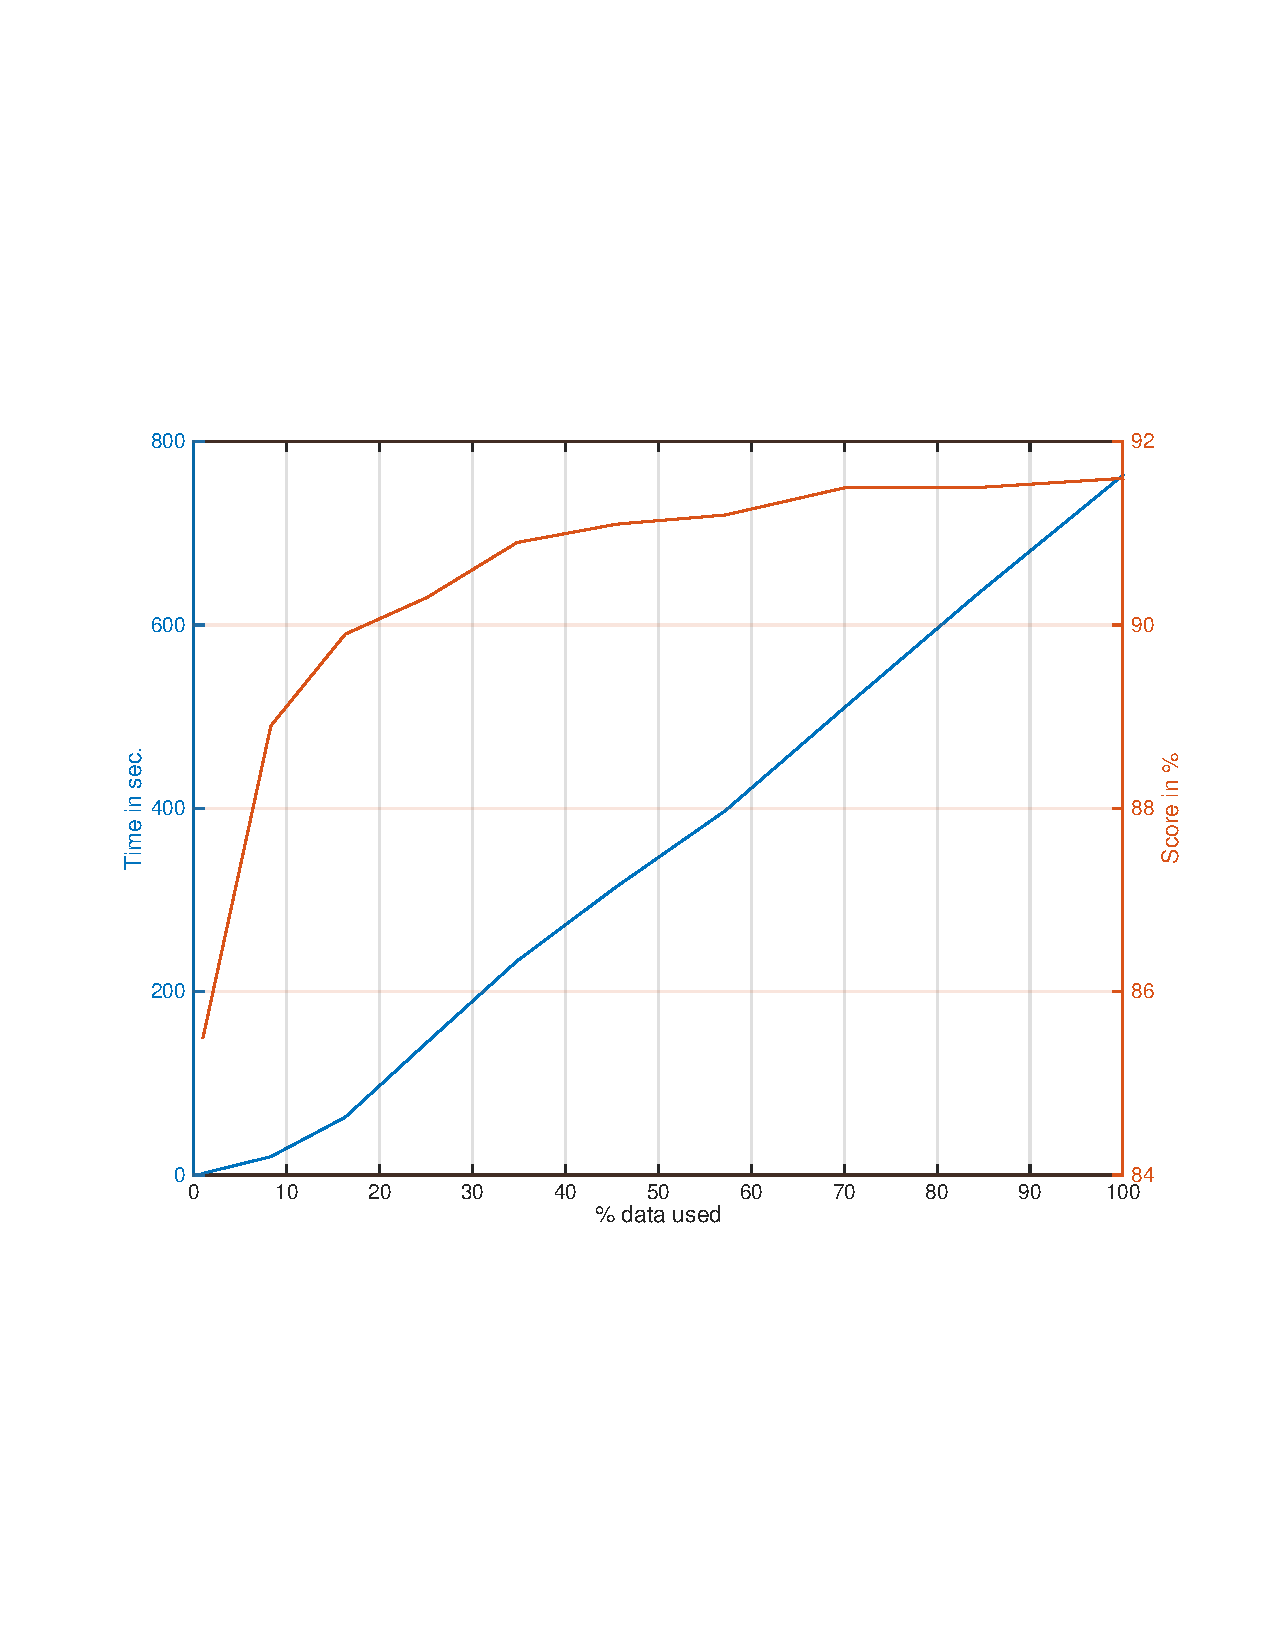
\includegraphics[trim=50 200 35 205,clip,width=\linewidth]{figures/lr_mnist.pdf}
  \caption{Logistic regression/MNIST}
  \label{sampledata1}
\end{subfigure}%
\begin{subfigure}{.45\textwidth}
  \centering
  \includegraphics[trim=50 200 35 205,clip,width=\linewidth]{figures/rf_mnist.pdf}
  \caption{Random forest/MNIST}
  \label{sampledata2}
\end{subfigure}
\begin{subfigure}{.45\textwidth}
  \centering
  \includegraphics[trim=50 200 35 205,clip,width=\linewidth]{figures/lr_synth.pdf}
  \caption{Logistic regression/synthetic data}
  \label{sampledata3}
\end{subfigure}
\begin{subfigure}{.45\textwidth}
  \centering
  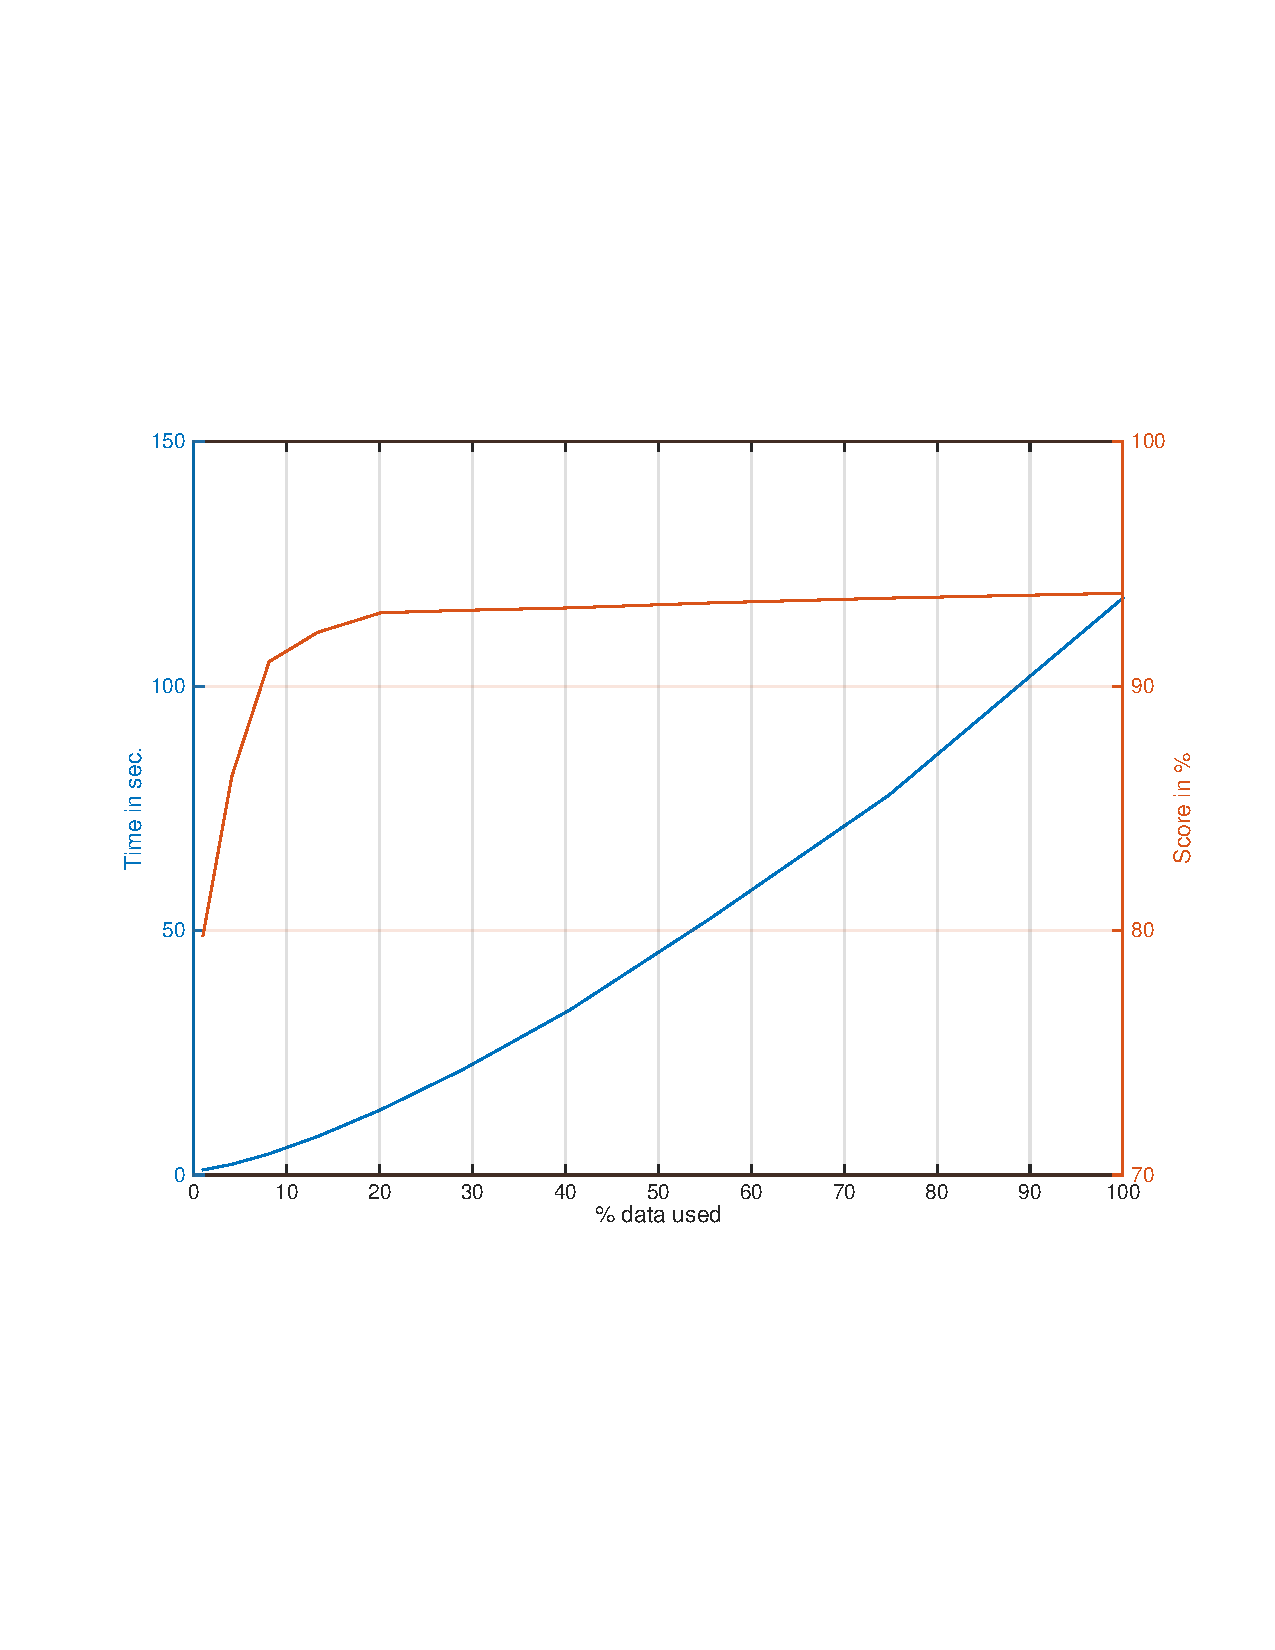
\includegraphics[trim=50 200 35 205,clip,width=\linewidth]{figures/rf_synth.pdf}
  \caption{Random forest/synthetic data}
  \label{sampledata4}
\end{subfigure}
\caption{Sample data plotting time (blue) and score (red) against the proportion of data used for four different algorithm/dataset combinations}
\label{sampledata}
\end{figure}



Figure \ref{sampledata} shows examples of collected performance data with the proportion of data as the approximation parameter shown on the $x$ axis. The four plots show the result of running random forests with 128 trees and logistic regression on the MNIST dataset and a synthetic dataset with $5,000$ samples and $500$ features (details on datasets used in this project can be found in the Evaluation chapter below).

In all four figures, the runtime, shown in blue, exhibits linear growth as the amount of data increases. Although the actual runtime of random forests is in $\mathcal{O}(n\ log\ n)$ instead of linear in the amount of data, we have found that in practice, it is still modelled well by a linear kernel. Since runtime values shown in Figure \ref{sampledata3} are substantially lower, the values are noisier than in the other graphs. 

The score (shown in red) for all four combinations of algorithms and datasets exhibits rapid growth in the beginning before levelling off. We model these curves with the exponential mixture kernel described in the next section.


\begin{figure}
\centering
\begin{subfigure}{.33\textwidth}
  \centering
  \includegraphics[trim=50 180 35 205,clip,width=\linewidth]{figures/2d_sample_data1.pdf}
  \caption{}
  \label{2d_1}
\end{subfigure}%
\begin{subfigure}{.33\textwidth}
  \centering
  \includegraphics[trim=50 180 35 205,clip,width=\linewidth]{figures/2d_sample_data2.pdf}
  \caption{}
  \label{2d_2}
\end{subfigure}
\begin{subfigure}{.33\textwidth}
  \centering
  \includegraphics[trim=50 180 35 205,clip,width=\linewidth]{figures/2d_sample_data3.pdf}
  \caption{}
  \label{2d_3}
\end{subfigure}
\caption{Three different perspectives on the same score data, plotting score against proportion of data used and the number of trees in a random forest on the amazon dataset}
\label{2d}
\end{figure}


Figure \ref{2d} shows a plot of random forests score data for two approximation parameters. The $x$-axis shows the number of decision trees, the $y$-axis the percentage of data used. The shape of the plot suggests a multiplicative relationship between the effect the two parameters have on the score.


\section{The Exponential Mixture Kernel}

Based on the sample data described in the previous section, we implemented a kernel to model the exponential behaviour of classification accuracy. Following \cite{2014arXiv1406.3896S}, we define the kernel as

\begin{align}
\kappa(x,x') &= \int_{0}^{\infty} e^{-\lambda x}e^{-\lambda x'}\mu(d\lambda)\\
&= \int_{0}^{\infty} e^{-\lambda(x+x')}\mu(d\lambda) \label{eq:kernel}
\end{align}

with $\mu$ being a mixing measure. The intuition for the integral shown in Equation \ref{eq:kernel} is that this kernel is computed as an infinite sum of exponential decay functions that form its basis functions. The weight of each of these basis functions is determined by the mixing measure $\mu$ whose parameters are the hyperparameters to the kernel.

Note that this kernel is not a stationary as $\kappa(x, x') \neq \kappa(x + \tau, x' + \tau)$. This conforms to our prior that moving further away from the origin, the value of $\kappa$ should decrease.

Again following \cite{2014arXiv1406.3896S}, we choose a gamma distribution as our mixing measure $\mu$, which leads to an analytic solution to the integral:
\begin{align}
\kappa(x, x') &= \int_0^{\infty} e^{-\lambda(x+x')}\frac{\beta^\alpha}{\Gamma(\alpha)}\lambda^{\alpha -1}e^{-\lambda\beta} d\lambda\\
&=\frac{\beta^\alpha}{\Gamma(\alpha)}\int_0^\infty e^{-\lambda(x+x'+\beta)}\lambda^{\alpha-1}d\lambda\\
&=\frac{\beta^\alpha}{(x+x'+\beta)^\alpha}
\end{align}

Diverging from \cite{2014arXiv1406.3896S}, we reparameterise the gamma distribution with
\begin{equation}
\psi = \mathbb{E}(x) = \frac{\alpha}{\beta}
\end{equation}
and
\begin{align}
\xi &= \frac{Var(x)}{\mathbb{E}^2 (x)} = \frac{\alpha}{\beta^2} \cdot \frac{\beta^2}{\alpha^2}\\
&= \frac{1}{\alpha}
\end{align}

\begin{figure}
\centering
\begin{subfigure}{.5\textwidth}
  \centering
  \includegraphics[trim=80 190 70 190,clip,width=0.95\linewidth]{figures/gamma_psi.pdf}
  \caption{Varying $\psi$, $\xi$ fixed at 1.1}
  \label{gammapsi}
\end{subfigure}%
\begin{subfigure}{.5\textwidth}
  \centering
  \includegraphics[trim=80 190 70 190,clip,width=0.95\linewidth]{figures/gamma_xi.pdf}
  \caption{Varying $\xi$, $\psi$ fixed at 1.1}
  \label{gammaxi}
\end{subfigure}
\caption{Varying the parameters to the reparameterised $\Gamma$-distribution}
\label{gammadist}
\end{figure}


Figure \ref{gammadist} shows how the reparameterised gamma distribution changes as $\psi$ and $\xi$ are varied. Note how the distributions Figure \ref{gammapsi} have the same shape with a different mean while the shape parameter $\xi$, shown in Figure \ref{gammaxi}, changes the shape of the distribution.

After reparameterisation, the term for the kernel becomes
\begin{equation}
\kappa(x, x') = \frac{\frac{1}{\psi\xi}^{\frac{1}{\xi}}}{(x+x'+\frac{1}{\psi\xi})^{\frac{1}{\xi}}}
\end{equation}

\begin{figure}
\centering

  \centering
  \includegraphics[trim=80 190 70 190,clip,width=.6\linewidth]{figures/expmix_psi1_xi1.pdf}
  \caption{Functions drawn from a Gaussian process with an exponential mixture kernel}
  \label{expmix11}
\end{figure}

Figure \ref{expmix11} shows functions drawn from a Gaussian process with the exponential mixture kernel as its covariance function. Note how these functions slowly decay to zero as $y$ grows.

The score functions we encounter in this project do not normally decay to zero, instead they plateau at values between 0 and 1. To model this effect, we add a constant function to the exponential mixture kernel in the fashion described in the Background chapter.

To model multi-dimensional data with multiple approximation parameters, we model every input dimension with a separate exponential mixture kernel and multiply these kernels together, adding a constant kernel to this product. To model each dimension with its own kernel, we use GPML's \texttt{covMask} utility kernel that allows masking out arbitrary input dimensions.

\section{Selecting Kernel Hyperparameters} 

To fit a Gaussian process to a given set of data points, one needs to find appropriate values for the hyperparameters to its covariance function. The two main ways to do so are marginalisation and optimisation. For reasons explained in the Evaluation chapter, we implement both of these methods in our project.

GPML includes an optimisation function called \texttt{minimize} that is meant to be used to optimise kernel hyperparameters. It relies on gradient information, which we implemented for the exponential mixture kernel. We were, however, not able to successfully optimise the hyperparameters to the exponential mixture kernel with this function, as the optimisation would terminate after a very small number of steps having moved only slightly from the initial values without having found a minimum. We suspect the reason for this to be numerical instability that creates small amounts of noise and creates tiny local minima that the optimiser is unable to escape from. 

Figure \ref{nlmlopt} shows a plot of a marginal likelihood function for data drawn from a Gaussian process prior that we tried to optimise with GPML's \texttt{minimize}. The plot strongly suggests that this is not a difficult function to optimise in principle.

\begin{figure}
\centering
  \centering
  \includegraphics[trim=60 190 70 190,clip,width=.6\linewidth]{figures/nlml_opt.pdf}
  \caption{The negative log marginal likelihood on a synthetic dataset of an exponential mixture kernel as a function of its first hyperparameter, $\psi$}
  \label{nlmlopt}
\end{figure}

After failing to optimise the hyperparameters to the exponential mixture kernel using the optimisation function included with GPML, we decided to implement a sampling method which does not suffer from the same problems as optimisation. After successfully implementing sampling, we decided to also write our own optimisation routine for reasons of speed and ease of use. Both methods are described in detail in the remainder of this section. An evaluation of the two methods applied to our data can be found in the Evaluation chapter.

\subsection{Sampling}
One approach to hyperparameter selection is the Bayesian approach of integrating out the hyperparameters $\theta$. Recall that the marginal likelihood given data $\mathcal{D}$, outputs $y$ and hyperparameters $\theta$ is defined as

\begin{equation}
p(\mathbf{y}|\mathcal{D}, \theta) = \int p(\mathbf{y}|f, \mathcal{D}, \theta)p(f|\mathcal{D}, \theta) df
\end{equation}

We can marginalise out $\theta$ from the marginal likelihood:

\begin{equation}
p(\mathbf{y}|\mathcal{D}) = \int p(\mathbf{y}|\mathcal{D}, \theta)p(\theta|\mathcal{D}) d\theta
\end{equation}

This integral can be approximated by sampling from $p(\theta|\mathcal{D})$ and calculating

\begin{equation}
p(\mathbf{y}|\mathcal{D}) \approx \sum p(\mathbf{y}|\mathcal{D}, \theta)p(\theta|\mathcal{D}) \Delta\theta
\end{equation}


The main advantage of sampling the hyperparameters is that it does not suffer from overfitting the way that optimisation does. Its major drawback is that it is computationally more expensive than optimisation methods. Sampling also takes more effort than optimisation to implement since the result of the computations the program executes have to be correctly averaged over.

\subsubsection{Slice sampling}

Slice sampling \cite{MacKay:2002:ITI:971143, neal2003} is a Markov Chain Monte Carlo (MCMC) sampling method. Sampling methods of this type generate samples by constructing a Markov chain that converges to the posterior distribution. The main advantage of slice sampling over other MCMC sampling methods is that it does not require careful tuning of its parameters which makes it particularly easy to use.

\begin{figure}[t]
\centering
  \includegraphics[trim=0 0 0 0,clip,width=\textwidth]{figures/slice_sampling.pdf}
  \caption{Slice sampling after having picked an $x'$ from the interval $(x_l,x_r)$ and before shrinking the interval}
  \label{slsamp}
\end{figure}

Given a distribution $f$ from which we want to sample, slice sampling samples by executing the following steps. We start at a point $x$ and evaluate $y = f(x)$. From the interval $(0, y)$, we uniformly draw a value $u$, the height of the slice that gives slice sampling its name. The next step is to span an interval $(x_l, x_r)$ around $x$. We subsequently draw $x'$ uniformly from this interval and calculate $y' = f(x')$. If $y' > u$, we return $x'$ as a sample. Otherwise we narrow the interval $(x_l, x_r)$ by setting $x'$ to be the new endpoint of the interval on the side of $x$ on which $x'$ falls.

Figure \ref{slsamp} shows slice sampling after the height $u$ of the slice has been chosen, the interval $(x_l, x_r)$ has been created and an $x'$ has been drawn from that interval. Since $f(x')$ is less than $u$, the next step of execution will shrink the interval by setting $x_r$ to $x'$.






\subsection{Optimisation}

Another approach to searching for suitable hyperparameters is to optimise the marginal likelihood of the model with respect to its hyperparameters:

\begin{equation}
\theta_{\text{opt}} = \argmax_\theta p(\mathbf{y}|\mathcal{D}, \theta)
\end{equation}


This has the advantage of being substantially faster than sampling. It is also easier to implement since it returns one set of hyperparameters that can be used to make predictions instead of multiple samples that have to be averaged over. The disadvantage of optimisation is that it is prone to overfitting by choosing one optimum in cases where multiple viable optima exist. We describe situations in which we encountered this problem in the Evaluation chapter, comparing optimised hyperparameters with the results of slice sampling.

As we had already successfully sampled hyperparameters using slice sampling as described above, we implemented an optimisation method that works similarly to how slice sampling draws samples. The first version of this algorithm is shown below in Algorithm \ref{opti1}.

\begin{algorithm}[t]
\begin{algorithmic}[1]
\Procedure{Optimise}{$f,x,iterations=100,width=1$}
\State $y\gets f(x),\ D\gets \Call{get\_dimensions}{x}$
\For{$i\gets 1, iterations$}
\For{$dim\gets \Call{permute}{D}$}\Comment{Iterate over all dimensions}
\State $x_l, x_r, x'\gets x$\Comment{$x_l,\ x_r$ span interval, $x'$ falls inside}
\State $r\gets \Call{Uniform}{0, 1}$
\State $x_l(dim)\gets x(dim) - r * width$
\State $x_r(dim)\gets x(dim) + (1 - r) * width$
\For{$j\gets 1, 15$}
\State $x'(dim)\gets \Call{Uniform}{x_r(dim), x_l(dim)}$
\State $y' = f(x')$
\If{$y' < y$}
\State $y\gets y',\ x(dim) = x'(dim)$\Comment{New optimum}
\Break
\EndIf
\If{$x'(dim) > x(dim)$}
\State $x_r(dim) = x'(dim)$\Comment{Narrow interval from the right}
\ElsIf{$x'(dim < x(dim)$}
\State $x_l(dim) = x'(dim)$\Comment{Narrow interval from the left}
\EndIf
\EndFor
\EndFor
\EndFor
\EndProcedure
\end{algorithmic}
\caption{First version of our custom optimisation routine}
\label{opti1}
\end{algorithm}

This optimisation algorithm starts at a given $x$ and optimises by iterating over the input dimensions, spanning up an interval around $x$ for every iteration. Inside of these iterations, it selects points $x'$ at random from the interval. If $f(x')$ is smaller than the current minimum, it sets $x(dim)$ to $x'(dim)$ and continues to the next loop iteration, otherwise it narrows the interval either from the left or the right, depending on the side of $x$ on which $x'$ falls.

Given sufficient data to fit to, this algorithm is able to find optimised hyperparameters to the exponential mixture kernel reliably. If it is used to fit a GP to a small number of points, it often selects hyperparameters such that the covariance matrix is not positive semidefinite and the Cholesky decomposition used in the inference algorithm fails. We catch these errors by wrapping every evaluation of $f$ in a \texttt{try ... catch} block in our Matlab code. 

While testing this algorithm, we found an effective method to handle these errors to be rerunning the algorithm multiple times and selecting the result with the highest marginal likelihood. This also alleviates the issue of local optima. The code to achieve this is shown in Algorithm \ref{optiwrap}.

\begin{algorithm}[h]
\begin{algorithmic}[1]
\Procedure{Optimise\_with\_restarts}{$f,x,restarts=5$}
\State $X \gets [\ ],\ Y \gets [\ ]$
\For{$i\gets 1, restarts$}
\State $x'\gets \Call{Optimise}{f, x}$
\State $y'\gets f(x')$
\State $\Call{append}{X, x'}$
\State $\Call{append}{Y, y'}$
\EndFor
\State \textbf{return} $X(\Call{MinIndex}{Y})$
\EndProcedure
\end{algorithmic}
\caption{Rerunning the optimisation routine}
\label{optiwrap}
\end{algorithm}

While this updated algorithm produces satisfying results, it takes substantially longer than the original version. A final change we therefore added was to terminate the optimisation routine early if the value of $y$ only changes by a small value $\epsilon$ over the course of five iterations. This condition is met during almost all executions and often drastically cuts short the time that our algorithm needs.

One shortcoming of this optimisation routine is that all its steps have to be axis aligned. If the gradient of the function being optimised at $x$ is not aligned with any axis, the optimiser will take small steps along multiple axes. A superior approach would be to directly move along the gradients, which are available to us. This would not be hard to implement because gradient information is available for the exponential mixture kernel. As our current algorithm already performs to a high standard, we did not investigate this potential improvement further. One other possible recent method that would improve on our current algorithm is described in \cite{DBLP:journals/corr/MahsereciH15}.



\chapter{Scheduling} 
\label{ch:scheduling}
\textit{This chapter describes the schedulers developed during the course of this project. It firsts gives a high level overview of the system architecture before describing the details of each of the schedulers.}

\section{System Architecture}

\subsection{High Level Architecture}
\begin{figure}[p]
    \centerline{\includegraphics[trim=40 90 35 90,clip,scale=0.8]{figures/architecture4.pdf}}
  \caption{High level architecture for one scheduler, shown after three iterations. Data is shown in green, machine learning algorithms in red and the scheduler in blue. Circled numbers refer to explanations in the text.}
    \label{architecture}
\end{figure}


Our system is designed in a two tiered fashion. Tier 1 creates models of the data using learning algorithms that are parameterised with approximation parameters. The training time and score of these models makes up the input to tier 2. This second layer first creates meta-models of the time and score of the models in tier 1. These meta-models are used by the scheduler to select the algorithm and approximation parameters for the next iteration and the process is repeated.

In this project, we focus on the two algorithms described in the Background chapter, random forests and logistic regression. These are two extremely common machine learning algorithms and are therefore well suited to demonstrate the feasibility of our methods. The approximation parameter we use in our evaluation is the percentage of the available data given to the learning algorithm to train a model. This decision was motivated by the fact that the proportion of data used is the clearest and most obvious way to run approximate version of an algorithm 

Figure \ref{architecture} shows this architecture diagrammatically for one scheduler after three iterations. In tier 1, the dataset \raisebox{.5pt}{\textcircled{\raisebox{-.9pt} {1}}} is used as input for all model creation. The learning process is parameterised by the learning algorithm and the approximation parameters to the algorithm \raisebox{.5pt}{\textcircled{\raisebox{-.9pt} {2}}}. The runtime time and score for every iteration are saved \raisebox{.5pt}{\textcircled{\raisebox{-.9pt} {3}}} separately for both algorithms.

In tier 2, this performance data is used to train four Gaussian processes \raisebox{.5pt}{\textcircled{\raisebox{-.9pt} {4}}}, two each for both algorithms. These Gaussian processes model the time and the score of the learning algorithms as the approximation parameter is varied. These meta-models form the input to the scheduler \raisebox{.5pt}{\textcircled{\raisebox{-.9pt} {5}}} that uses them to make a decision on an algorithm/approximation parameter combination for the next iteration \raisebox{.5pt}{\textcircled{\raisebox{-.9pt} {6}}}.


\begin{lstlisting}[caption=The main loop of our scheduling program with slight edits for readability, label=mainloop]
while True:
    terminate = True

    for scheduler in schedulers:
        scheduler.decide()
        if scheduler.decision:
            terminate = False
            
            scheduler.execute()
            if scheduler.needs_model():
                scheduler.model() 
            scheduler.draw()

    if terminate:
        break
\end{lstlisting}


Note how both tiers execute machine learning algorithms (coloured in red) on data (coloured in green) and how the results of the algorithms in the first tier form the dataset for the Gaussian Processes in tier 2. The main loop of our program is shown, slightly simplified, in Listing \ref{mainloop}.

\begin{figure}[p]
    \centerline{\includegraphics[trim=70 120 50 120,clip,scale=0.475]{figures/system_example.pdf}}
  \caption{The program running with three schedulers}
    \label{systemexample}
\end{figure}

Figure \ref{systemexample} shows the program running with three schedulers. Rows one to three are each one instance of the architecture depicted in Figure \ref{architecture}; the plot in row four compares the performance of the three schedulers. For the three running instances, the first column shows runtime information. Logistic regression data is shown in blue while random forest data is shown in red. The dots represent recorded data points, the blue line shows the mean of the model that predicts runtime while the shaded area is twice the standard deviation of the model, showing the model's uncertainty. The scheduler shown in row one does not require models to make decisions and only shows the recorded data points. For schedulers that operate on time budgets, this plot also shows how much time is currently remaining by drawing a black line at the time threshold.

The plot in the second column shows the score data and model in the same way the runtime information is displayed in the first column. Additionally, for schedulers that model time and score (the second and third in Figure \ref{systemexample}), the acquisition functions for both algorithms are shown as dashed lines. The precise shape of these functions depends on the strategy the scheduler uses to make decisions. To decide which algorithm to evaluate next with how much data, the scheduler calculates the maximum of both acquisition functions.

The third row contains plots of the score against the time as a point cloud for logistic regression (blue) and a random forest (red). These point clouds are created by drawing 100 points each from the time and score model and plotting one against the other. Again, these plots are only computed for schedulers that model performance data.



\subsection{Directory Structure of the Code}

The directory of the project contains the following subdirectories:
\begin{itemize}
\item \textbf{data/}: This directory contains the datasets in \texttt{data/raw\_arffs/} and data generated by the sample data generation scripts is stored here. When creating plots based on this sample data, the results are also written to this folder
\item \textbf{figs/}: Every diagram our system displayes is automatically also saved to this directory
\item \textbf{report}/: This folder is where the source file and diagrams for this document are stored
\item \textbf{src/}: This directory holds the source code for our project. It contains \texttt{main.py}, the main file and two subdirectories, \texttt{src/data\_handling/} and \texttt{src/matlab/} which contain Python and Matlab code respectively
\item \textbf{var/}: This folder is used to store temporary files that are used to exchange data between the part of our system written in Python and the part written in Matlab
\end{itemize}



\subsection{Interoperability between Python and Matlab}
Choosing Matlab to implement the performance modelling code and Python to implement the other parts of our system made it necessary to devise a method of transferring data between these two parts of the program. During the initial planning stage, we intended to write all parts of the system in Python but the advantages of GPML, such as level of documentation and ease of use, later outweighed the disadvantages of having to implement process interoperability.

To start the program, \texttt{main.py} is executed. \texttt{main.py} calls the Matlab script that contains modelling code whenever it has collected new data and needs to update one of its performance models. Data is transferred between the Python and the Matlab scripts by writing it to \texttt{json} files\footnote{JSON is a widespread data format similar to XML.} in the \texttt{var/} directory.  Before the Matlab script is executed, \texttt{main.py} writes the recorded performances of the algorithm for which it has just updated its data to \texttt{var/scheduler\_data.json}. This file contains a JSON object with the fields \texttt{x\_percent\_data}, \texttt{y\_times} and \texttt{y\_scores} which hold the data collected so far.

Once it has finished modelling the performance data, the Matlab script writes the models to \texttt{var/models.json} and terminates. This file contains an array of model objects. These models are represented as 100 linearly spaced data points between 0\% and 100\% of available data. They each have an \texttt{m} and an \texttt{sd} field for the mean and standard deviation respectively. This file is read by \texttt{main.py} and the old models are overwritten with the updated ones.


\section{Implemented Schedulers}
\begin{figure}
    \centerline{\includegraphics[trim=55 70 35 55,clip,width=\linewidth]{figures/scheduler_inheritance.pdf}}
  \caption{The inheritance structure of the implemented schedulers. Abstract schedulers are shown in italics set on grey}
    \label{schedulerinheritance}
\end{figure}

Every scheduler is implemented as a separate class of which there are nine in total. There are three abstract scheduler classes that implement functionality shared between two or more schedulers while the other six implement scheduling strategies that can be used to schedule data collection. The last two schedulers described in this chapter form a novel contribution while the others are implemented as baselines for purposes of comparison and as intermediate steps to the more advanced schedulers.

The inheritance structure of the scheduler classes is shown in Figure \ref{schedulerinheritance}. In this section, we describe each scheduler's functionality before describing their behaviour and comparing them in the Evaluation chapter.

\subsection{\texttt{\textit{Scheduler}}}
This is the base class that every scheduler inherits from. It defines a framework of functionality that all schedulers share. Besides drawing routines and code to write performance and read model data, this class contains the following methods:

\begin{itemize}
\item \texttt{\_\_init\_\_}: the class constructer initialises a number of properties, including the \texttt{self.data} property which holds an array of learning performances for each algorithm
\item \texttt{decide}: this is an abstract method that is called to decide on the next algorithm/approximation parameter combination to be evaluated. It sets the \texttt{self.decision} property of the scheduler object. If the scheduler is done, either due to having finished optimising or because its time budget has been used up, this property is set to \texttt{None}
\item \texttt{execute}: this method executes the decision made by the \texttt{decide} method and adds the new time and score to the \texttt{self.data} property
\item \texttt{model}: this function updates the model for the algorithm for which data was collected during the last execution of the \texttt{execute} method. It reads the value of the \texttt{self.decision} property to determine this algorithm and is called after \texttt{execute} finishes
\end{itemize}



\subsection{\texttt{FixedSequenceScheduler}}
The \texttt{FixedSequenceScheduler} is the simplest of all the scheduling strategies implemented. Its constructor expects an array of data percentage values and computes the cartesian product of the learning algorithms with this array. When its \texttt{decide} method is called, it writes the next element of this product into \texttt{self.decision}, cycling through algorithms and executing the fixed sequence of data percentage values. Once it has executed every algorithm/data percentage combination, the scheduler terminates.

This scheduler is unique among the schedulers in not requiring a model of runtime and score. Its evaluation sequence is set during initialisation and it does not rely on predictions to decide which learning algorithm/approximation parameter combination to try next.


\subsection{\texttt{\textit{ProbablisticScheduler}}}

This is the base class of all schedulers that make probabilistic decisions using an acquisition function as described in the Background chapter. Its constructor expects an array that contains values for the approximation parameter used during a burn-in phase. During this phase, the scheduler collects initial performance data and does not create models of the performance data.

This scheduler has an abstract class method \texttt{a} that takes a time and score model (expressed as arrays of mean and standard deviation) and calculates the acquisition function. If slice sampling was used to integrate out the hyperparameters to the exponential mixture kernel, \texttt{\textit{ProbablisticScheduler}} is responsible for calling \texttt{a} as many times as there are samples and averaging over the resulting acquisition functions. Time and score model samples are taken independently which allows us to randomly pair one time and one score model per iteration.

\subsection{\texttt{ProbabilityOfImprovementScheduler}}
This is the simplest concrete probabilistic scheduler. It implements the probability of improvement heuristic for Bayesian optimisation. As mentioned in the Background chapter, this is not an optimal scheduling strategy. It is, however, still included for purposes of comparison.

This scheduler truncates its acquisition function at the maximum $x$ value at which data has been collected for each algorithm and only considers percentage of data values that are strictly greater than the current maximum. This encodes the assumption that using more data can never produce a model worse than the current best.

\subsection{\texttt{ExpectedImprovementScheduler}}
\texttt{ExpectedImprovementScheduler} implements the Ex\-pec\-ted im\-prove\-ment heu\-ris\-tic for Bayesian optimisation. Like the previous scheduler, it truncates its acquisition function and only considers using more data than before for subsequent execution of the learning algorithms.

\subsection{\texttt{ExpectedImprovementPerTimeScheduler}}
This scheduler inherits from the \texttt{ExpectedImprovementScheduler} and differs from it only by dividing the expected improvement by the mean of the time model. This calculates the expected improvement per unit of time and biases it towards faster executions of the learning algorithms, even if the improvement over the current best is not as large as slower executions.

\subsection{\texttt{\textit{TimedScheduler}}}
\texttt{\textit{TimedScheduler}} is the base class of the two schedulers that operate on a finite time budget. It inherits from \texttt{\textit{ProbablisticScheduler}} and includes functionality to keep track of the remaining time. It also adds a line to the time plot to mark how much time is left.

\subsection{\texttt{ExpectedImprovementTimesProbOfSuccessScheduler}}
This scheduler is the first of the two schedulers that form a main contribution of this project. It inherits from both the \texttt{\textit{TimedScheduler}} and the \texttt{ExpectedImprovementScheduler}. To compute its acquisition function, it multiplies the expected improvement with the probability of successfully finishing the learning process in the remaining time. The probability of success for a given $x$ value, i.e. the probability of finishing model creation within the remaining time, is calculated by cutting off the normal distribution of the time model at $x$ and computing the amount of remaining probability mass. Formally:

\begin{equation}
p_{\text{success}}(x) = \Phi(\frac{t - \mu_{\text{time}}(x)}{\sigma_{\text{time}}(x)})
\end{equation}

where $t$ is the remaining time.

The constructor of the \texttt{ExpectedImprovementTimesProbOf\-Success\-Scheduler} expects a sequence of time intervals. Whenever the scheduler has used up its available time budget, the next time interval in the sequence is added to the remaining time until the all available time has been used up.

\subsection{\texttt{MinimeseUncertaintyAndExploitScheduler}}
The \texttt{MinimeseUncertaintyAndExploitScheduler} is the second main scheduler of this project. It inherits from \texttt{\textit{TimedScheduler}} and has two scheduling phases, exploration and exploitation. Each phase is alloted a separate time budget. In the first phase, it tries to build adequate models by reducing uncertainty. Its acquisition function during this phase is calculated as the score model standard deviation divided by the time it takes to evaluate the function at the point under consideration.

After using up the time allocated for exploration, this scheduler uses the second time budget to construct the best model it can within that time, using the knowledge it obtained during the first phase. In this phase the acquisition function is calculated as the mean of the score model times the probability of success.


\chapter{Evaluation}

\textit{This chapter describes the results of our project and evaluates the system we built. It also lists challenges that we faced during its development and limitations it currently has.}

\section{Datasets}
The first set of datasets we used was created synthetically using scikit-learn's \texttt{make\_classification} function. This function takes a number of parameters that define the dataset, such as the number of samples, the number of features and the number of classes and creates data according to these parameters. 

This fine grained control over the properties of the datasets was valuable to us, as it allowed us to see how our system handles datasets of different nature. We wrote a small script\footnote{Saved at \texttt{src/data\_handling/dataset\_creator.py}} to enable us to quickly create datasets and see how logistic regression and random forests perform on subsets of these datasets.


A second set of datasets was drawn from the list of datasets that were used in the development of Auto-WEKA which we mentioned in the Related Work chapter. The authors of Auto-WEKA made the datasets that were used to test Auto-WEKA available on their website\footnote{They can be downloaded at http://www.cs.ubc.ca/labs/beta/Projects/autoweka/datasets/}.

These datasets originally came from a variety of sources \cite{Lichman:2013, Larochelle:2007:EED:1273496.1273556, Krizhevsky09learningmultiple} and were converted by the Auto-WEKA creators to WEKA's own data format, the Attribute-Relation File Format (\texttt{arff}). This made it convenient for us to use these datasets since they are originally in a wide range of differing data formats. If we had downloaded them from their original sources, they would have had to be converted manually. 

Besides converting them to the \texttt{arff} format, the authors of the Auto-WEKA paper also split them up into a training and a test set. As described in the Implementation chapter, we use k-fold cross-validation in this project and therefore needed all samples in a single file. To achieve this, a small ruby script\footnote{Saved at \texttt{src/data\_handling/utils/append\_arff\_files.rb}} was written to merge the \texttt{train.arff} and \texttt{test.arff} files for each dataset.

While some of the datasets in this collection are entirely numerical, some have textual features while still others have a mixture of strings and numbers as features. An example of this is the \texttt{germancredit} dataset, which has a feature \texttt{credit\_history} with possible values that include \texttt{"all paid"} and \texttt{"critical/other existing credit"}. It also has a feature called \texttt{age} that is of type integer.

When using these datasets, we load the \texttt{arff} files into memory using SciPy's \texttt{scipy.io.arff.loadarff} function. As scikit-learn expects all features to  be numerical, we convert features that are not numerical using a technique called one-of-k encoding.

This encoding expands every feature of type string with $n$ possible values into $n$ boolean typed features. This means that a feature that can take discrete, non-numerical values, such as \texttt{other\_payment\_plans}, also taken from the \texttt{germancredit} dataset, with possible values \texttt{bank}, \texttt{stores} and \texttt{none} is encoded as three separate features, \texttt{other\_payment\_plans=bank}, \texttt{other\_payment\_plans=stores} and \texttt{other\_payment\_plans=none}. For every sample in the dataset, one of these features is be set to $1$ and all others to $0$, according to the value of \texttt{other\_payment\_plans}.

Table \ref{datasets_info} lists the names and sizes of the datasets used. It includes both synthetic and real-world data. Small and large datasets are separated with small datasets at the top and large datasets at the bottom of the table.


\begin{table}[t]
\centering


\begin{tabular}{|l|l|l|l|}
\hline
Dataset          & \# samples & \# features & \# classes \\ \hline\hline
Abalone          & 4,177       & 8           & 28         \\ \hline
Amazon           & 1,500       & 10,000       & 50         \\ \hline
Car              & 1,728       & 6           & 4          \\ \hline
Germancredit     & 1,000       & 20          & 2          \\ \hline
Krvskp           & 3,196       & 36          & 2          \\ \hline
Madelon          & 2,600       & 500         & 2          \\ \hline
Semeion          & 1,593       & 256         & 10         \\ \hline
Shuttle          & 58,000      & 9           & 7          \\ \hline
Waveform         & 5,000       & 40          & 3          \\ \hline
Winequalitywhite & 4,898       & 11          & 7          \\ \hline
Yeast            & 1,484       & 8           & 10         \\ \hline\hline
MNIST            & 62,000      & 784         & 10         \\ \hline
Synthetic1            & 10,000       & 500           & 2         \\ \hline
Synthetic2            & 10,000       & 1,000           & 2         \\ \hline
Synthetic3            & 20,000       & 1,500           & 2         \\ \hline
Synthetic4            & 40,000       & 2,000           & 2         \\ \hline
\end{tabular}

\caption{Datasets used for evaluation with large datasets shown at the bottom}
\label{datasets_info}

\end{table}

\section{Model Comparison}
In this section, we assess the quality of the fits to score data the exponential mixture kernel achieves. We do so by comparing the marginal likelihoods of the models it generates to those of a kernel that encodes weaker prior knowledge about the shape of the data, the squared exponential kernel.




\begin{table}[t]
\centering
	\begin{tabular}{|l|l|l|l|}
\hline
Dataset          & Exp. mixt. nlml & Sq. exp. nlml & Bayes factor \\ \hline\hline
Abalone          & \textbf{-37.984}  & -34.138  & 3.846         \\ \hline
Amazon           & \textbf{-24.641}  & -21.769  & 2.872         \\ \hline
Car              & \textbf{-30.685}  & -25.251  & 5.434         \\ \hline
Germancredit     & \textbf{-27.806}  & -23.858  & 3.948         \\ \hline
Krvskp           & \textbf{-33.710}  & -30.226  & 3.484         \\ \hline
Madelon          & -24.786           & \textbf{-25.212} & -0.426  \\ \hline
Semeion          & \textbf{-32.969}  & -27.234  & 5.735         \\ \hline
Shuttle          & \textbf{-45.728}  & -44.317  & 1.411         \\ \hline
Waveform         & \textbf{-38.294}  & -27.317  & 10.977        \\ \hline
Winequalitywhite & \textbf{-34.842}  & -32.331  & 2.511         \\ \hline
Yeast            & -28.428           & \textbf{-28.676} & -0.248  \\ \hline\hline
MNIST            & \textbf{-46.028}  & -37.350  & 8.678         \\ \hline
Synthetic1       & \textbf{-30.107}  & -11.668  & 18.439        \\ \hline
Synthetic2       & \textbf{-24.622}  & -11.661  & 12.961        \\ \hline
Synthetic3       & \textbf{-19.479}  & -15.978  & 3.501        \\ \hline
Synthetic4       & \textbf{-16.761}  & -7.059   & 9.702         \\ \hline
\end{tabular}

	\caption{The negative log marginal likelihoods of fitting an exponential mixture kernel and a squared exponential kernel to logistic regression score data}
\label{log_reg_fits}
\end{table}


\begin{table}[t]
\centering
\begin{tabular}{|l|l|l|l|}
\hline
Dataset          & Exp. mixt. nlml & Sq. exp. nlml & Bayes factor \\ \hline\hline
Abalone          & -                 & -       & -              \\ \hline
Amazon           & \textbf{-20.737}  & -18.355 & 2.382          \\ \hline
Car              & \textbf{-27.436}  & -24.440 & 2.996          \\ \hline
Germancredit     & \textbf{-24.955}  & -23.857 & 1.098          \\ \hline
Krvskp           & \textbf{-35.775}  & -27.289 & 8.486          \\ \hline
Madelon          & \textbf{-24.589}  & -23.921 & 0.668          \\ \hline
Semeion          & \textbf{-22.272}  & -18.516 & 3.756          \\ \hline
Shuttle          & \textbf{-50.859}  & -47.183 & 3.676          \\ \hline
Waveform         & \textbf{-32.038}  & -27.309 & 4.729          \\ \hline
Winequalitywhite & \textbf{-27.074}  & -24.302 & 2.772          \\ \hline
Yeast            & \textbf{-24.474}  & -23.146 & 1.328          \\ \hline\hline
MNIST            & \textbf{-41.603}  & -30.850 & 10.753         \\ \hline
Synthetic1       & \textbf{-25.364}  & -13.954 & 11.410          \\ \hline
Synthetic2       & \textbf{-25.224}  & -14.714 & 10.511         \\ \hline
Synthetic3       & \textbf{-20.865}  & -15.708 & 5.158          \\ \hline
Synthetic4       & \textbf{-22.730}   & -10.559 & 12.171         \\ \hline
\end{tabular}
	\caption{The negative log marginal likelihoods of fitting an exponential mixture kernel and a squared exponential kernel to random forest score data}
\label{rnd_forest_fits}
\end{table}

Tables \ref{log_reg_fits} and \ref{rnd_forest_fits} show negative log marginal likelihoods of fits using both kernels to score data for our test datasets. As described in the Background chapter, the squared exponential kernel only encodes a smoothness prior and is commonly used as a baseline against kernels that encode stronger priors.

When using the negative log marginal likelihood, smaller values indicate a better fit. To compare the marginal likelihoods for the two kernels, we compute the Bayes factor which is defined as the quotient of the two marginal likelihoods. Since our marginal likelihoods are expressed in log-space, this is equal to the difference between the values for each kernel. The Bayes factor is to be interpreted as a measure of how much better one model fits the data than the other. Greater values for the Bayes factor are better in our case, as they express a better fit of the exponential mixture kernel.

In Tables \ref{log_reg_fits} and \ref{rnd_forest_fits}, we have grouped our datasets into small and large datasets again, separated by a double line. As can be seen from inspecting the tables, the Bayes factors for the large datasets are substantially larger than those for smaller datasets. This is due to the fact that the score data for small datasets tends to be much noisier which obscures the exponential nature of the data.

Figure \ref{madelon_logreg_fit} shows the two fits for the madelon dataset random forest score data with the squared exponential kernel shown in blue and the exponential mixture kernel shown in red. The data, shown as black crosses, is so noisy, that the optimiser was not able to find a sensible fit for the exponential mixture kernel.

Figure \ref{synth3_rndforest_fit} shows the two fits for the Synthetic3 dataset, where the exponential mixture kernel, again shown in red, achieves a much better fit than the squared exponential kernel. For $x$ values that lie beyond the data  available, the exponential mixture kernel makes confident predictions that conform to our expectation of having reached a plateau.


Our results show that the exponential mixture kernel is an appropriate choice to model the score data for large datasets where it achieves a substantially better fit than the squared exponential kernel. We do not consider the weaker performance of the exponential mixture kernel on score data for small datasets a significant weakness. The justification for this is that the problems that we attempt to make a contribution towards solving with this project, namely approximateness trade-offs when learning, do not usually arise when there is little data since in those cases, it is normally feasible to simply use all the available data, as doing so will take little time.

\begin{figure}[h]
\centering
\begin{subfigure}{.45\textwidth}
\centering
  \includegraphics[trim=50 200 50 190,clip,width=\textwidth]{figures/madelon_logreg_fit.pdf}
  \caption{Fits for the madelon logistic regression score data. The data is so noisy that the program is not able to find sensible hyperparameters to the exponential mixture kernel.}
  \label{madelon_logreg_fit}
\end{subfigure}
\begin{subfigure}{.45\textwidth}
\centering
  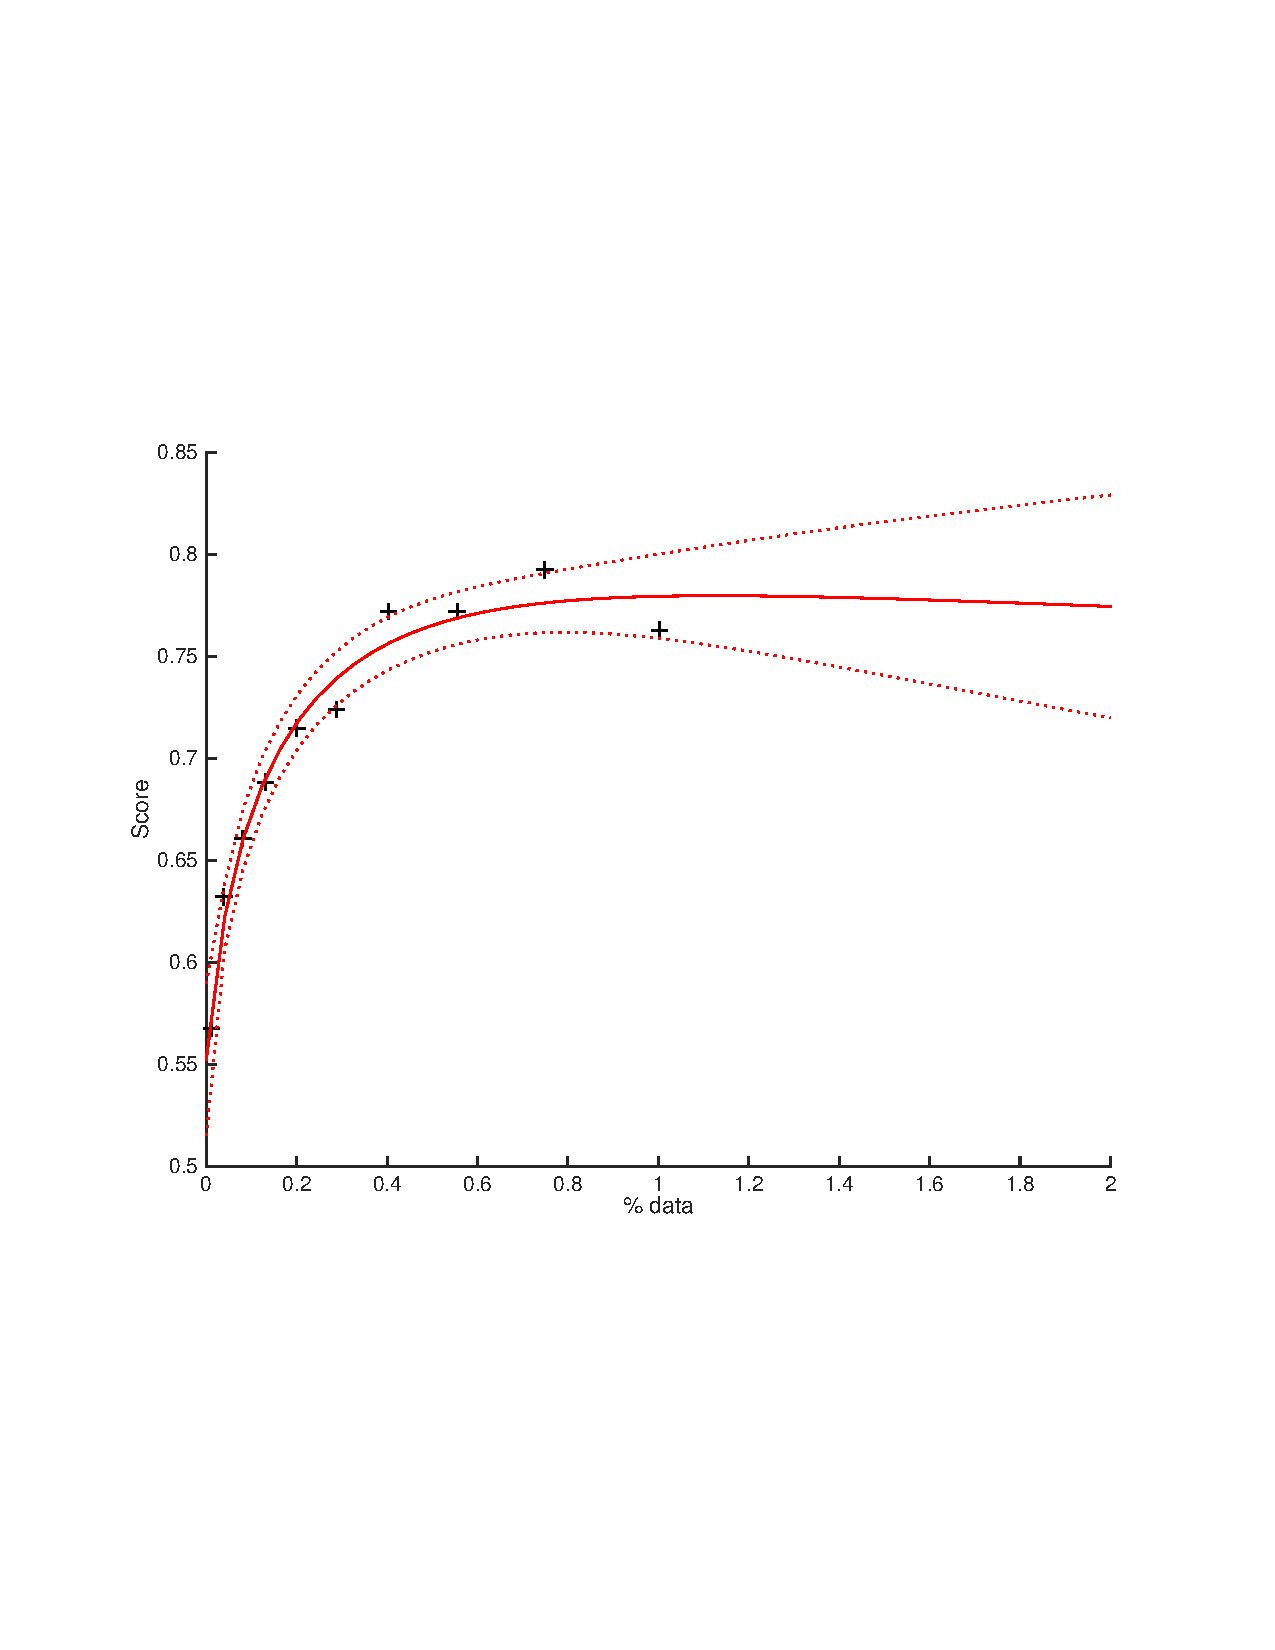
\includegraphics[trim=50 170 50 200,clip,width=\textwidth]{figures/synth3_rndforest_fit.pdf}
  \caption{Fits for the Synthetic3 logistic regression score data with the squared exponential fit in blue and the exponential mixture fit in red.}
  \label{synth3_rndforest_fit}
\end{subfigure}
\caption{Sample fits. The squared exponential fit is shown in blue and the exponential mixture fit in red}
\label{fits}
\end{figure}

\section{The Exponential Mixture Kernel}

\subsection{Hyperparameter Selection}

We generally found both of the methods we use for hyperparameter selection, sampling and optimisation, to return satisfactory results. As is in its nature, however, optimisation is prone to overfitting. This happens when there are multiple likely interpretations of the data reflected in multiple optima of the marginal likelihood. Optimisation can only choose one of these optima and becomes overconfident in one particular interpretation of the data.

\begin{figure}[t]
\centering
\begin{subfigure}{.45\textwidth}
  \centering
  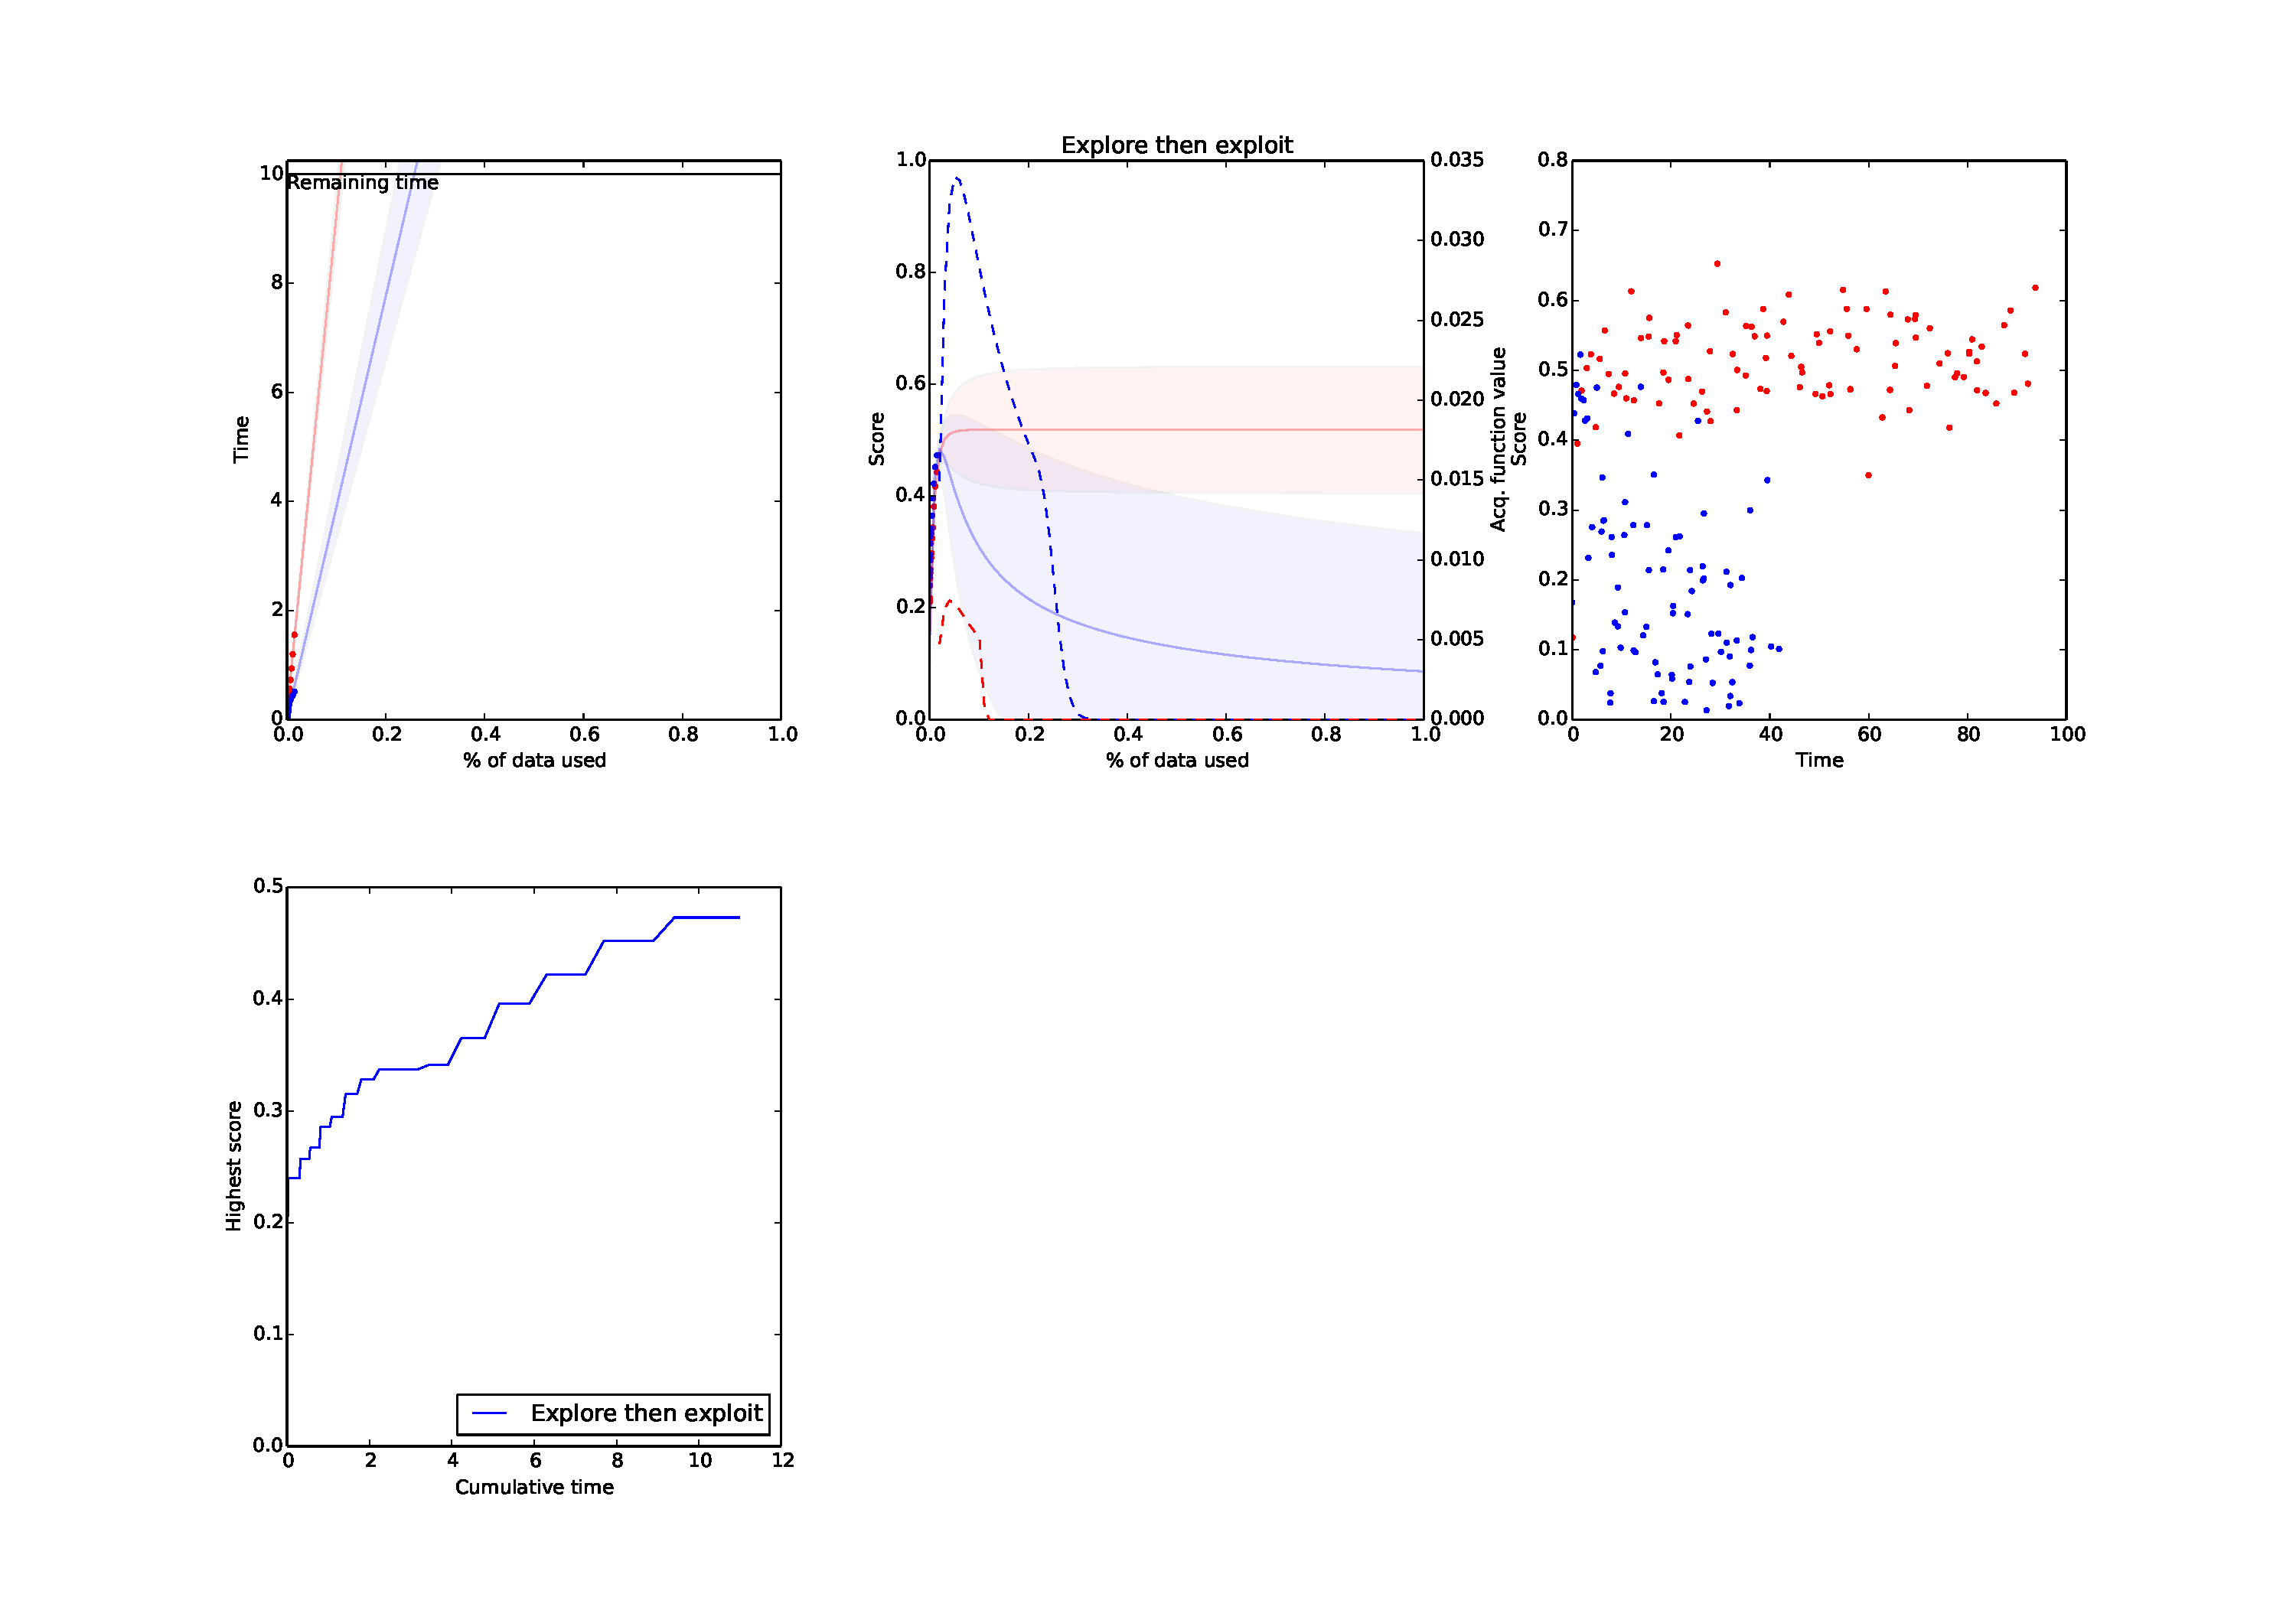
\includegraphics[trim=540 520 493 80,clip,width=\textwidth]{figures/kernel_issues1.pdf}
\caption{The blue mean sharply decreases for predicted $x$ values when we expect it to increase}
  \label{kernel_issues1}
\end{subfigure}%
\begin{subfigure}{.45\textwidth}
  \centering
  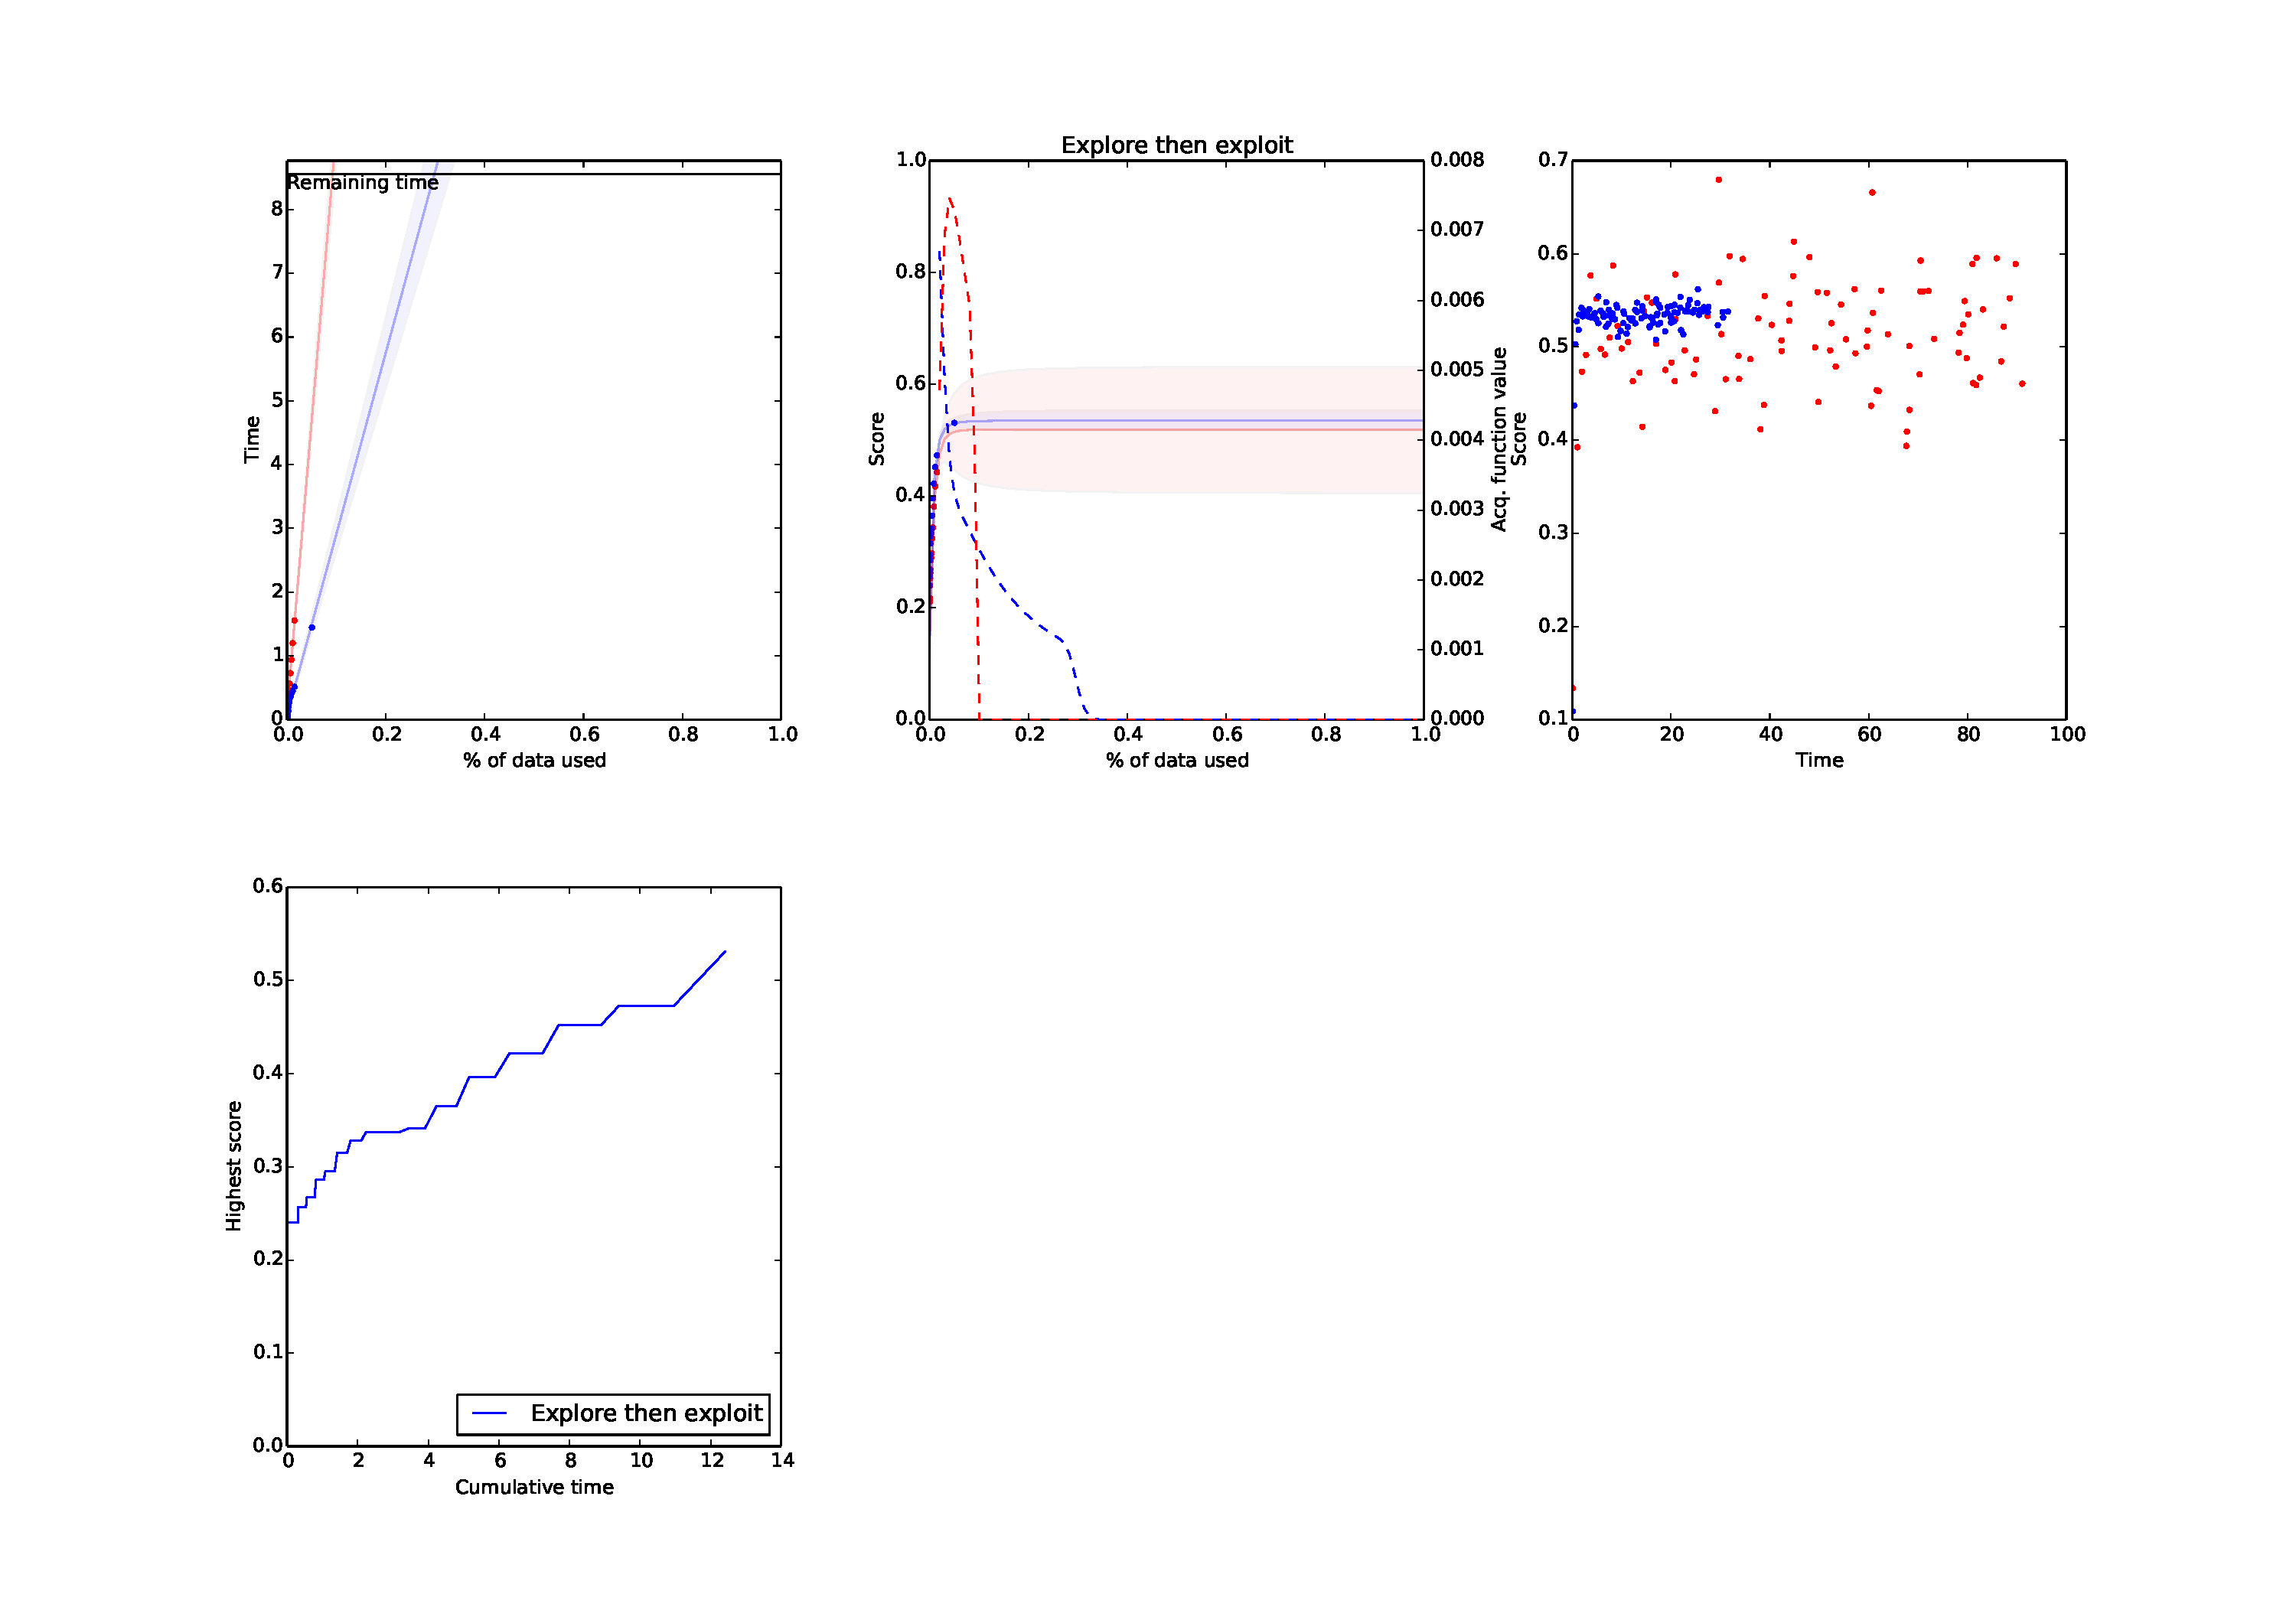
\includegraphics[trim=540 520 493 80,clip,width=\textwidth]{figures/kernel_issues2.pdf}
  \caption{Both means have flat shapes unlikely to be correct and the blue model's variance is too low}
  \label{kernel_issues2}
\end{subfigure}
\caption{Optimisation issues}
\label{kernel_issues_big1}
\end{figure}

\begin{figure}[p]
\centering
  \includegraphics[trim=540 710 500 75,clip,width=.9\textwidth]{figures/kernel_issues3.pdf}
  \caption{The red model completely fails to model the exponential nature of the data}
  \label{kernel_issues3}
\end{figure}

\begin{figure}[p]
\centering
  \includegraphics[trim=540 360 493 370,clip,width=.9\textwidth]{figures/sampling_example.pdf}
  \caption{An example of models with sampled hyperparameters}
  \label{sampling_example}
\end{figure}

This is an issue especially in the early phases of data collection after a few iterations when only little data was available. We addressed this problem by increasing the number of data points collected during the burn-in phase. As the subsets used in this phase are a small percentage of the whole dataset, this only adds marginally to the time spent in the burn-in stage.

Although this solved the issue of overfitting on too little data, sampling hyperparameters still proved more robust. Figures \ref{kernel_issues_big1} and \ref{kernel_issues3} show cases where optimisation fails to return sensible results.

Due to its faster speed, we mostly used optimisation while evaluating our system. From a theoretical perspective, however, the speed of hyperparameter selection is insignificant as it does not grow with the size of the datasets and gets dominated by the time spent on model construction.

Since our program has to be able to handle both samples and single sets of hyperparameters as returned by optimisation, our implementation treats the result of our optimisation routine as a single sample. This makes it completely transparent to the routines that use performance models, which of the two hyperparameter selection methods were used and enables us to switch between them freely depending on the requirements of the schedulers.

Figure \ref{sampling_example} shows models that are obtained by sampling hyperparameters. Every solid red and blue line is the mean of one model. To compute the red acquisition function for random forests, the acquisition functions for all red models are computed and averaged over. The acquisition function for logistic regression is computed equivalently.



\section{Scheduling Results}

\subsection{Scheduler Behaviour}

\subsubsection{\texttt{FixedSequenceScheduler}}
\begin{figure}[h]
\centering
  \includegraphics[trim=130 275 507 510,clip,width=\textwidth]{figures/fixed_sequence_example.pdf}
  \caption{A fixed exponential sequence}
  \label{fixedsequenceexample}
\end{figure}

Figure \ref{fixedsequenceexample} shows a \texttt{FixedSequenceScheduler} with a geometric sequence of data percentage values after about 25 iterations. In the previous iteration, it trained a logistic regression model with 80\% of the available data (the rightmost blue dots on both subplots) and is about to create a random forest model with the same amount of data.

This scheduler does not model performance data and does not adjust its decisions during the course of its execution.


\subsubsection{\texttt{ProbabilityOfImprovementScheduler}}
\begin{figure}[t]
\centering
  \includegraphics[trim=530 496 545 296,clip,width=\textwidth]{figures/prob_of_imp_01.pdf}
  \caption{Probability of improvement acquisition function}
  \label{sched:probofimpr1}
\end{figure}

The \texttt{ProbabilityOfImprovementScheduler} tends to be slow and conservative in exploring the function. Figure \ref{sched:probofimpr1} shows the score models and the acquisition functions for both algorithms as dashed lines. Although the model it has of logistic regression score data has a higher mean for all $x$ values, the scheduler is less certain about how the score of this algorithm changes as $x$ grows compared to random forests. Consequently, it will create a random forest model next.

\begin{figure}[p]
\centering
  \includegraphics[trim=530 270 547 510,clip,width=\textwidth]{figures/prob_of_imp_02.pdf}
  \caption{Probability of improvement acquisition functions}
  \label{sched:probofimpr2}
\end{figure}

\begin{figure}[p]
\centering
  \includegraphics[trim=530 710 545 55,clip,width=\textwidth]{figures/prob_of_imp_03.pdf}
  \caption{Probability of improvement acquisition functions after the scheduler has finished}
  \label{sched:probofimpr3}
\end{figure}

Figure \ref{sched:probofimpr2} shows a situation similar to the one shown in Figure \ref{sched:probofimpr1}. The uncertainty in this case, however, is roughly equal for both algorithms. The acquisition functions behave accordingly with the acquisition function for random forests being lower because it is less likely to improve over the current maximum $y$ which was achieved by logistic regression.



In Figure \ref{sched:probofimpr3}, we see the final state of a probability of improvement scheduler. The small step size at which it created logistic regression models is a typical behaviour of this scheduler. 

\subsubsection{\texttt{ExpectedImprovementScheduler}}


Figure \ref{sched:expimpr01} shows typical acquisition functions for the \texttt{Expected\-Improvement\-Scheduler}. Recall that the expected improvement strategy automatically balances exploration and exploitation, and that both, a high mean and a high variance increase the value of the acquisition function. Figure \ref{sched:expimpr01} demonstrates this effect: while the mean of both meta-models for $x$ values greater than about 0.4 are almost equal, the expected improvement for random forests overtakes the one for logistic regression because its variance is greater.

\begin{figure}
\centering
  \includegraphics[trim=530 710 493 55,clip,width=\textwidth]{figures/expimpr01.pdf}
  \caption{Expected improvement acquisition functions}
  \label{sched:expimpr01}
\end{figure}



\subsubsection{\texttt{ExpectedImprovementPerTimeScheduler}}
\begin{figure}
\centering
  \includegraphics[trim=140 710 493 55,clip,width=\textwidth]{figures/ei_by_time_1.pdf}
  \caption{Expected improvement per time performance models and acquisition function}
  \label{sched:expimprpertime01}
\end{figure}

The \texttt{ExpectedImprovementPerTimeScheduler} is a slight variation of the \texttt{ExpectedImprovementScheduler}. To calculate its acquisition function, it divides the expected improvement by the mean of the time model. Figure \ref{sched:expimprpertime01} shows the bias this scheduler has towards models that can be created quickly. Although the expected improvement increases as $x$ becomes larger, the required time also grows (shown in the left plot). This causes the acquisition function for logistic regression to have its peak at around $0.3$.


\subsubsection{\texttt{ExpectedImprovementTimesProbOfSuccessScheduler}}

This is one of two schedulers that expect to be given a time budget during initialisation. Figure \ref{sched:expimprtimeprob01} shows the state of the scheduler with one second to spend after the burn-in phase has finishd. This time limit is marked on the left plot. As can be seen on that plot, the probability that creating a random forest model with more than about 10\% of data will finish in time is extremely low. Consequently, the acquisition function for random forests is essentially flat and not visible on the right plot.

\begin{figure}[h]
\centering
  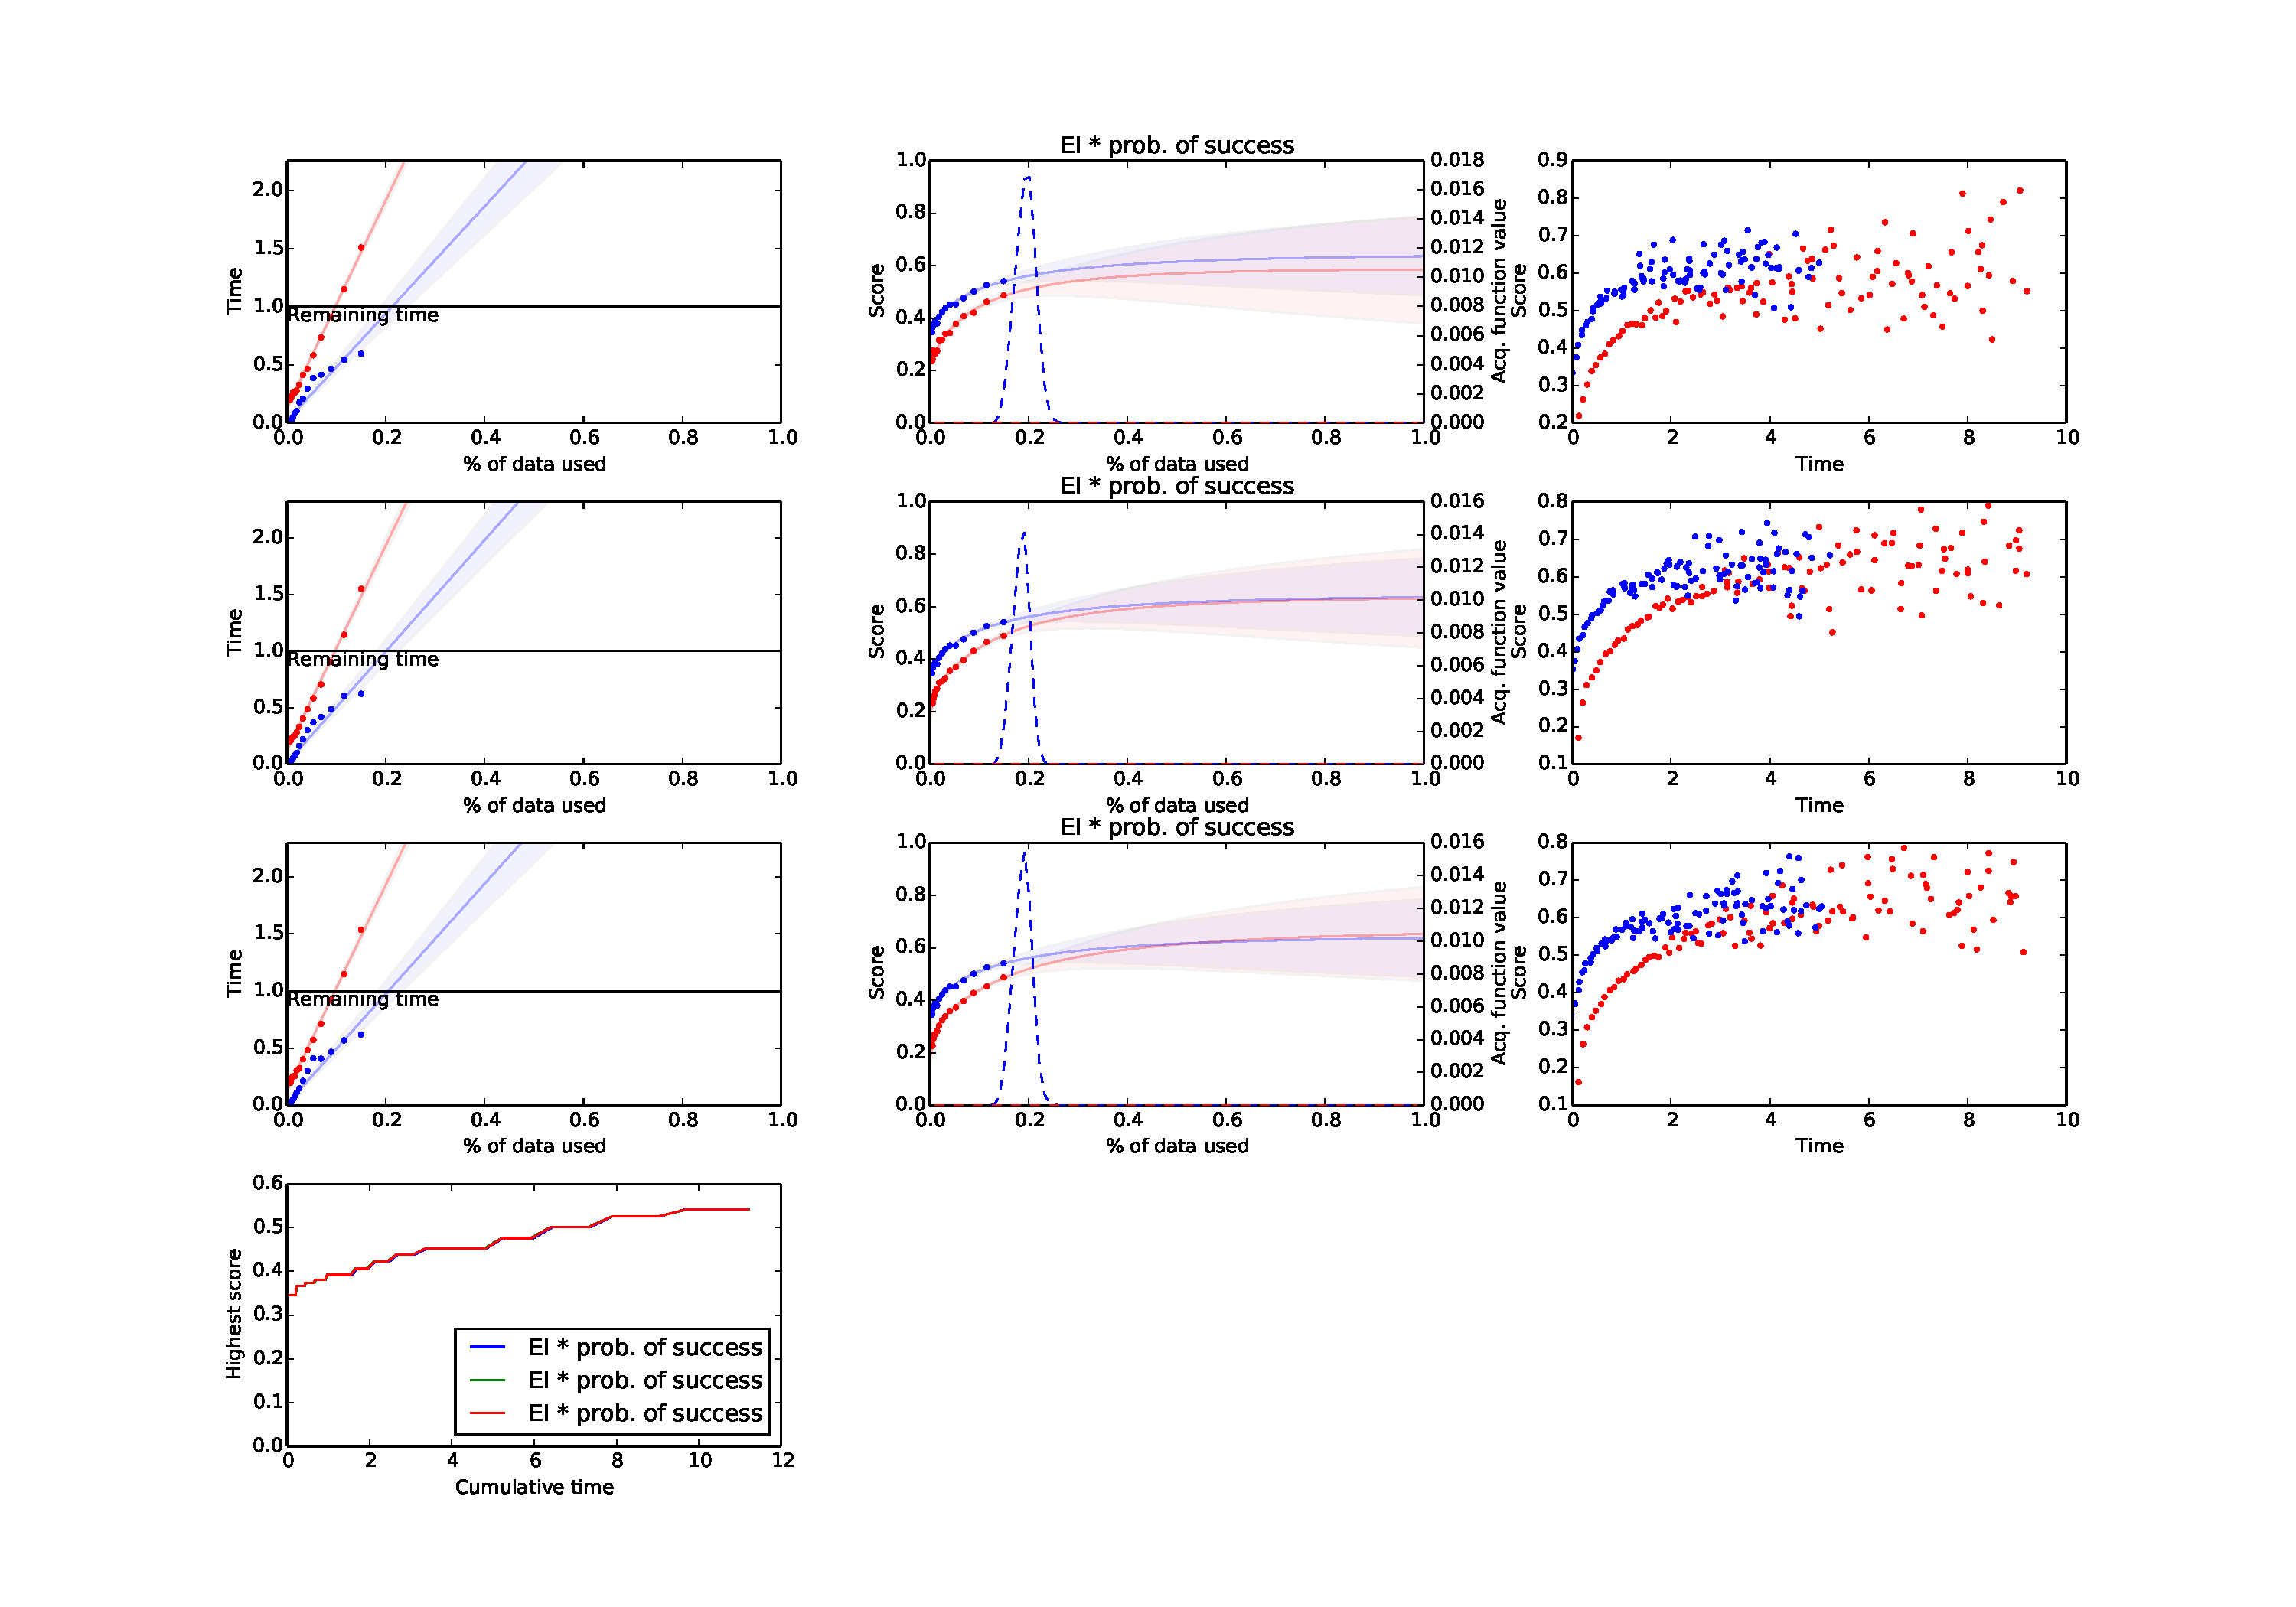
\includegraphics[trim=140 710 493 55,clip,width=\textwidth]{figures/ei_probofsuccess1.pdf}
  \caption{Expected improvement times probability of success after the burn-in period with an initial time budget of one second}
  \label{sched:expimprtimeprob01}
\end{figure}

The acquisition function of logistic regression algorithm with its peak around 0.2 reflects that the fact that the time model predicts that creating a logistic regression model with 20\% of the data will take about one second. For values larger than that, the probability of success rapidly decreases.

\begin{figure}
\centering
  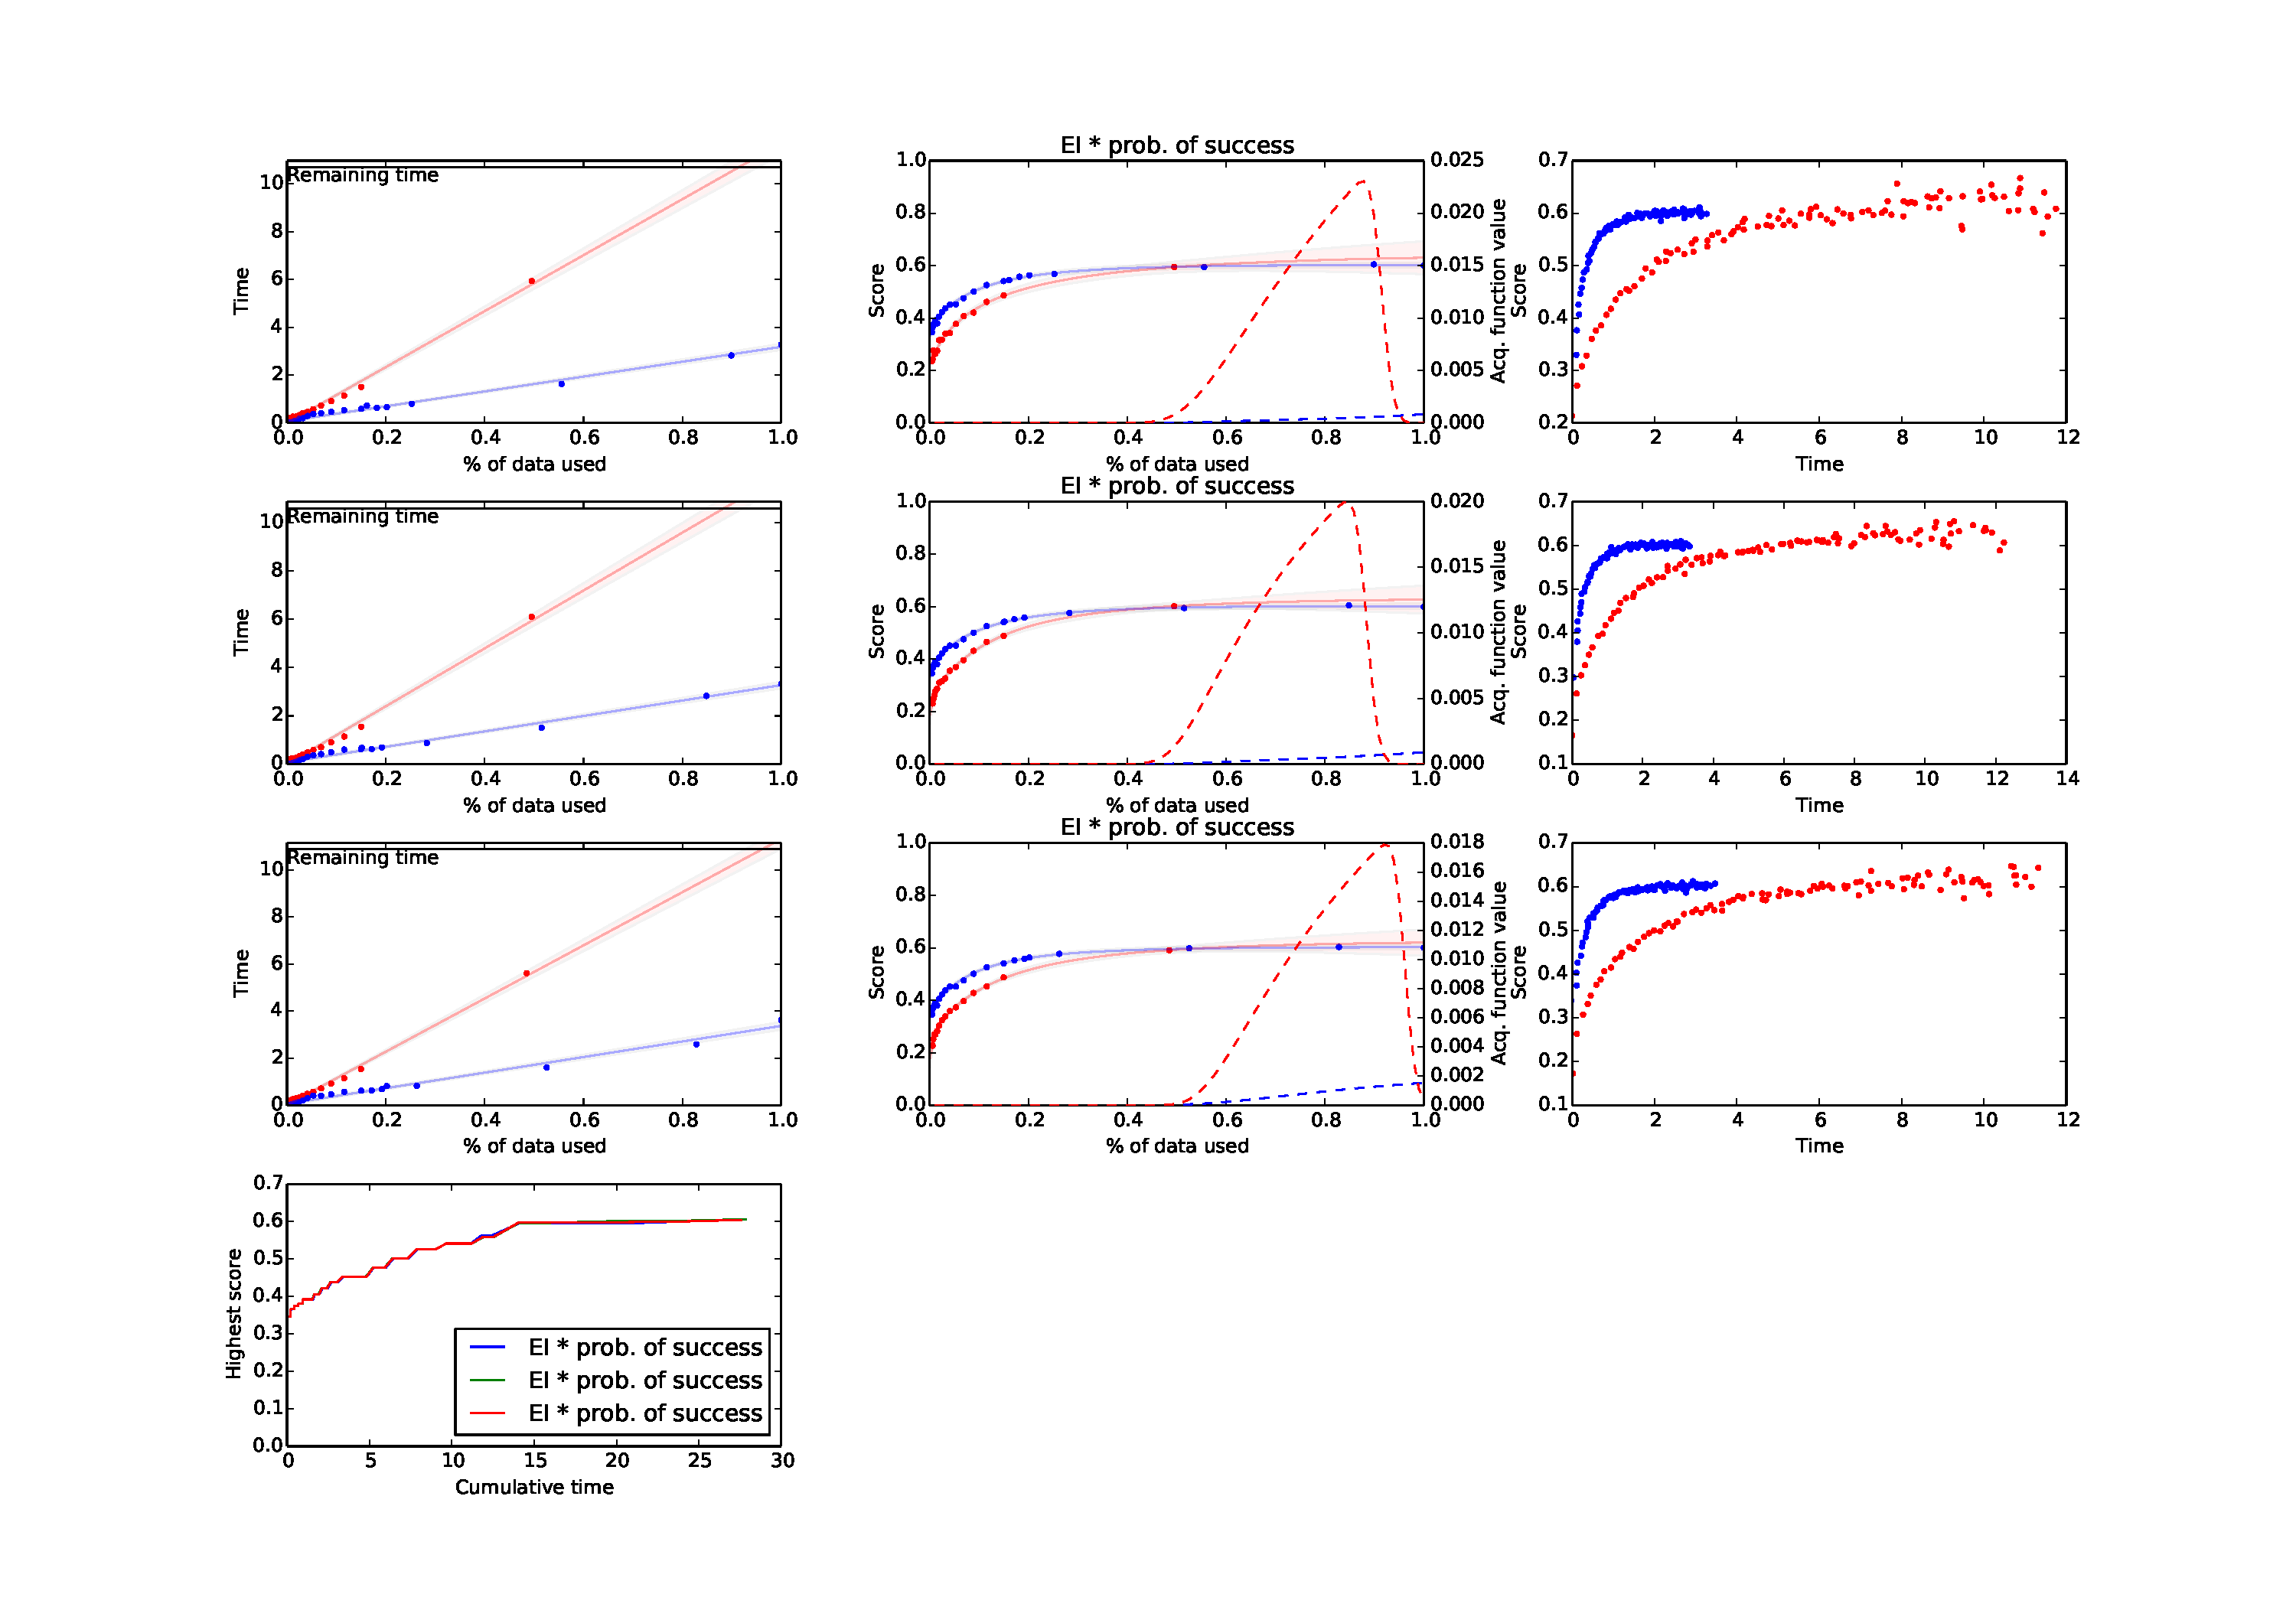
\includegraphics[trim=140 710 493 55,clip,width=\textwidth]{figures/ei_probofsuccess2.pdf}
  \caption{Expected improvement times probability of success at a later state of execution}
  \label{sched:expimprpertime02}
\end{figure}

Figure \ref{sched:expimprpertime02} shows the \texttt{ExpectedImprovementTimesProbOfSuccessScheduler} at a later stage of execution. Logistic regression models have been created with several subsets of the data and the scheduler does not expect much improvement by creating another logistic regression model. It has about 12 seconds to spend on building a random forest model. The runtime of this algorithm exceeds the time budget for $x$ values close to 1, which is reflected in the sharp drop-off in the acquisition function on the right at around an $x$ value of $0.9$.

\subsubsection{\texttt{MinimeseUncertaintyAndExploitScheduler}}

The \texttt{MinimeseUncertaintyAndExploitScheduler} is the second scheduler implemented in this project that operates on a time budget. Recall that it functions in two stages, exploration and exploitation, that are each allocated time during initialisation.

Figure \ref{sched:exp_then_exp1} shows the scheduler shortly after the burn-in period has finished. To illustrate the behaviour of this scheduler, we use a much larger dataset with $50,000$ samples. We use sampling instead of optimisation for hyperparameter selection in this example.

The scheduler is given 10 seconds to explore and 30 to exploit the knowledge gained during exploration. Due to the size of the dataset, it is not possible to build a model using all the available data in 30 seconds. This makes it necessary for the scheduler to be strategic about where it spends the time allocated for exploitation.

In Figure \ref{sched:exp_then_exp1}, random forests has, on average, higher variance in its scores than the blue algorithm. It takes longer to evaluate, however, which causes its acquisition function to have smaller values as the scheduler computes it as $\sigma/\text{time} \cdot \text{probability of success}$. Note how the acquisition functions for both algorithms sharply drop off as the projected time exceeds the current time budget of about 9 seconds. This point is reached for random forests at 0.1 and at 0.2 for logistic regression.


\begin{figure}
\centering
  \includegraphics[trim=140 710 493 55,clip,width=\textwidth]{figures/exp_then_exp1.pdf}
  \caption{``Minimise uncertainty and exploit" heuristic after burn-in has finished}
  \label{sched:exp_then_exp1}
\end{figure}

Figure \ref{sched:exp_then_exp2} shows the scheduler at the next iteration. A logistic regression model has been trained with about 8\% of the available data. The decrease in variance around this point is clearly visible in the blue acquisition function which has a valley around this point. Now, the large variance of the random forest model causes the red acquisition function to dominate, even though it quickly drops off as the predicted runtime for random forests exceeds the remaining exploration time of about 7 seconds.

\begin{figure}
\centering
  \includegraphics[trim=140 710 493 55,clip,width=\textwidth]{figures/exp_then_exp2.pdf}
  \caption{``Minimise uncertainty and exploit" heuristic after creating a logistic regression model}
  \label{sched:exp_then_exp2}
\end{figure}


In Figure \ref{sched:exp_then_exp3}, the scheduler has created a random forest model at the point where the red acquisition function shown in Figure \ref{sched:exp_then_exp2} has its maximum. This required all the remaining exploration time and the scheduler has now transitioned to the exploration phase. This is reflected in the remaining time which has been set to 30 seconds. Using this time, the scheduler tries to create the best model it can using its time budget, calculated as the score mean times the probability of success.

\begin{figure}[h]
\centering
  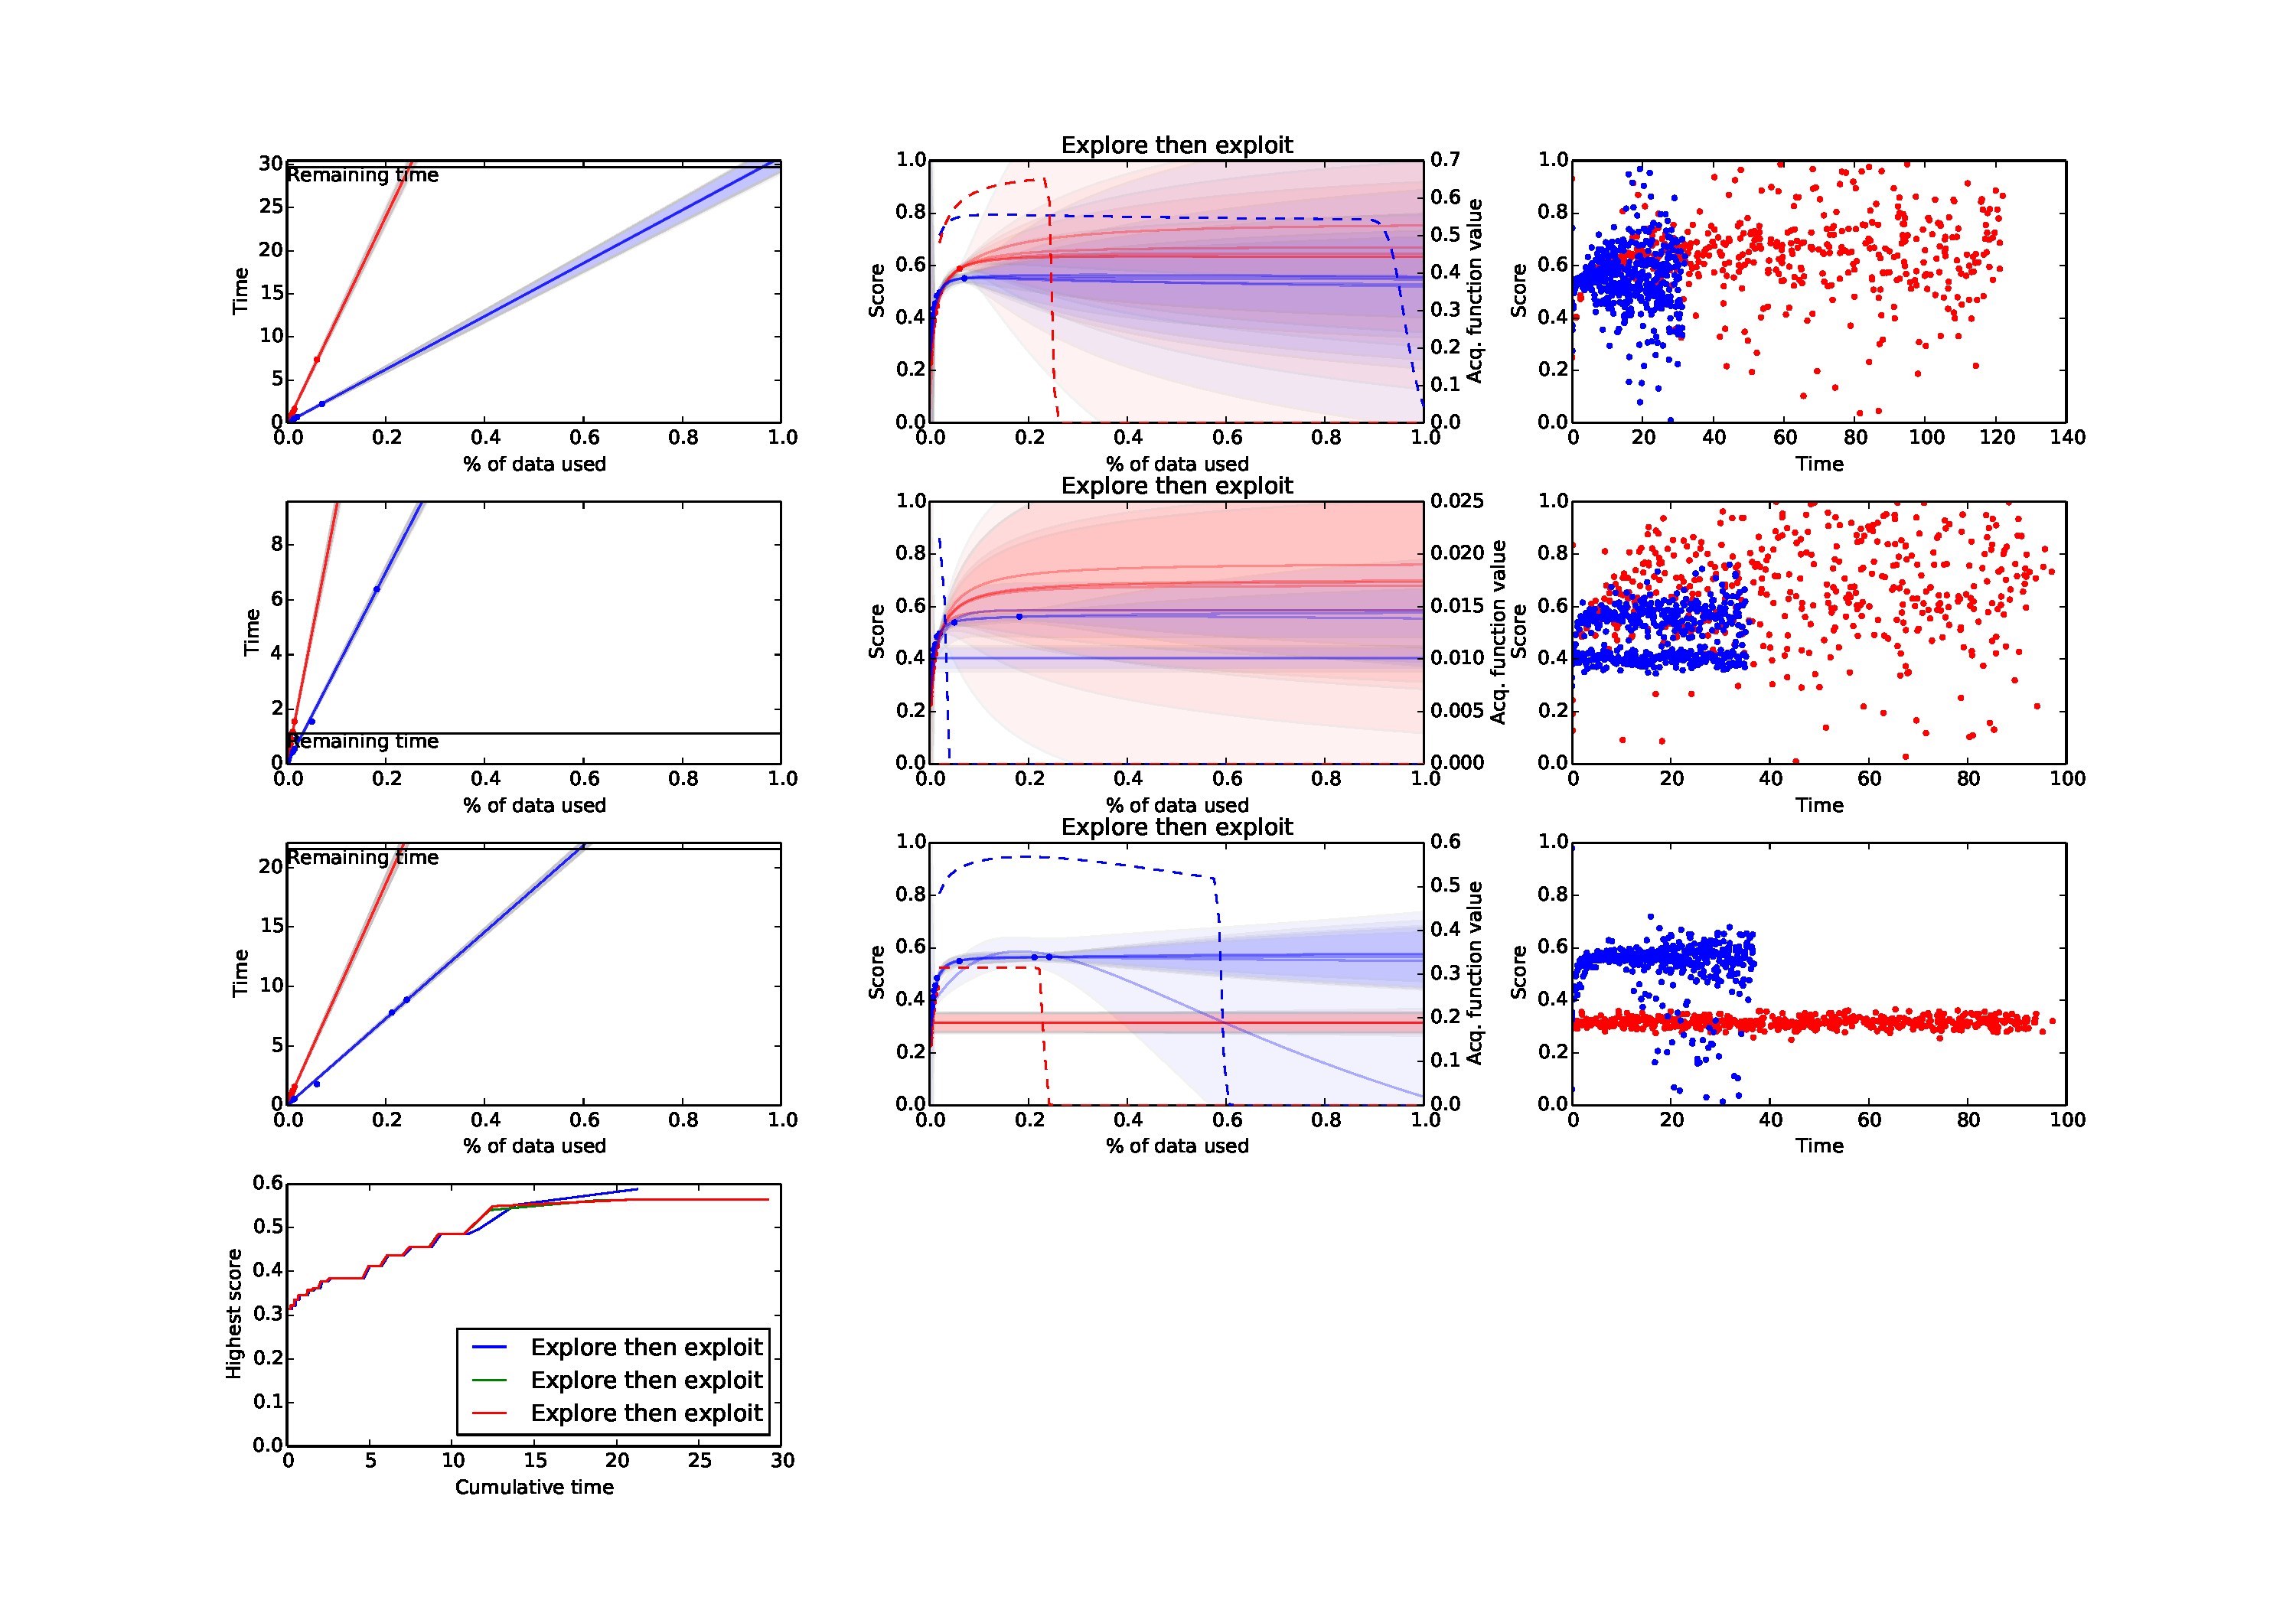
\includegraphics[trim=140 710 493 55,clip,width=\textwidth]{figures/exp_then_exp3.pdf}
  \caption{The exploitation phase of the ``minimise uncertainty and exploit" heuristic}
  \label{sched:exp_then_exp3}
\end{figure}

The acquisition functions for both logistic regression and random forests reflect the mean of the means of the sampled score models until the predicted time exceeds 30 seconds and the probability of success quickly goes to zero. The scheduler predicts the best model to be a random forest model created with about 23\% of the available data.





\subsection{Scheduler Performance}
In this section, we evaluate the heuristics for the two approximation trade-off goals described in the introduction to this report: anytime and contract algorithms.


\subsubsection{Anytime algorithm}

\begin{figure}[h]
\centering
  \includegraphics[trim=0 0 0 0,clip,width=.6\textwidth]{figures/constructed_dataset_anytime.pdf}
  \caption{Score data for one of the datasets used to test the anytime heuristic chosen for the fact that at different proportions of data, different algorithms create superior models}
  \label{constructed_dataset_anytime}
\end{figure}

Figure \ref{constructed_dataset_anytime} shows score data for a synthetic dataset with 7,500 samples, 120 features and 6 classes. This dataset has the noteworthy property that while a random forest model on the full data achieves a higher score than a logistic regression model, if we restrict ourselves to 50\% or less of the samples, logistic regression beats random forests.


\begin{figure}
\centering
  \includegraphics[trim=110 50 895 650,clip,width=.6\textwidth]{figures/anytime2.pdf}
  \caption{The highest score over time for two schedulers}
  \label{anytime2}
\end{figure}



Figure \ref{anytime2} shows the result of comparing our anytime heuristic, the \texttt{Expected\-Improvement\-Times\-Prob\-OfSuccessScheduler}, against a baseline of a \texttt{Fixed\-Sequence\-Scheduler} for this dataset. When the burn in period ends after about 25 seconds, the \texttt{Expected\-ImprovementTimesProbOfSuccessScheduler} immediately constructs much better models than the \texttt{Fixed\-Sequence\-Scheduler}. Eventually, both schedulers reach 100\% of data with both random forests and logistic regression, at which point they achieve the same score\footnote{In Figure \ref{anytime2}, the last model the \texttt{FixedSequence\-Scheduler} scheduler creates is slightly better than that of the \texttt{Expected\-Improvement\-Times\-Prob\-Of\-Success\-Scheduler}. This is due to the variance in random forest models.}.




\subsubsection{Contract algorithm}

We reuse the dataset shown in Figure \ref{constructed_dataset_anytime} to test our contract heuristic, using only 5,000 of the 7,500 samples, however, which moves the point at which random forests overtakes logistic regression to about 65\% of data.

We first test our contract heuristic, the \texttt{Minimese\-Uncertainty\-And\-Exploit\-Scheduler}, with an exploration time budget of 5 seconds and an exploitation time budget of 12 seconds. After finishing exploring, it has reached the state shown in Figure \ref{explexlp0_1}. The acquisition functions shown on the right plot form the basis for the decision it makes next: where to spend its exploitation time. The heuristic predicts that at 80\% of data, a random forest model will be better than the logistic regression model it created in the last iteration.

\begin{figure}[p]
\centering
  \includegraphics[trim=120 510 500 40,clip,width=\textwidth]{figures/explexlp0_1.pdf}
  \caption{The \texttt{MinimeseUncertaintyAndExploitScheduler} after finishing exploring}
  \label{explexlp0_1}
\end{figure}

\begin{figure}[p]
\centering
  \includegraphics[trim=120 510 500 40,clip,width=\textwidth]{figures/explexlp0.pdf}
  \caption{The \texttt{MinimeseUncertaintyAndExploitScheduler} after finishing exploiting}
  \label{explexlp0}
\end{figure}

The final state of the scheduler is shown in Figure \ref{explexlp0}. The scheduler has spent its exploration time budget gaining more knowledge on the runtime of logistic regression but, using the models it has of the score, decided to spend the time available for exploitation building a random forest model.





Figure \ref{explexlp1} shows the final state of running a \texttt{Minimese\-Uncertainty\-And\-Exploit\-Scheduler} on another synthetic dataset with $50,000$ samples, $80$ features and $5$ classes, giving it 30 seconds to explore and 60 seconds to exploit. It chose to spend its exploitation time budget on constructing a random forest model with about 40\% of the available data. It correctly predicted the time it would take to build this model based on the runtime meta-model it constructed during the exploration phase. This can be seen on the left plot, with the rightmost data point at an $x$ values of 0.4 marking the final model having taken exactly one minute to build.

\begin{figure}
\centering
  \includegraphics[trim=140 495 493 297,clip,width=\textwidth]{figures/explexlp1.pdf}
  \caption{The \texttt{MinimeseUncertaintyAndExploitScheduler} after finishing exploiting}
  \label{explexlp1}
\end{figure}



Although our anytime and contract heuristics have limitations which we describe in the next section, they still perform to a high standard. The results described above would be difficult for a human expert to reproduce by hand.

\subsection{Limitations}
One limitation of our current system is that it models the function from approximation parameters to runtime as linear in all cases. Not all machine learning algorithms, however, have linear runtimes. Using the two algorithms that we restricted ourselves to in this project, we have found a linear model to be adequate for empirical purposes. However, if the system is to be extended to other algorithms that have runtimes that are not well modelled by a linear kernel, such as Support Vector Machines with a runtime of $\mathcal{O}(n^3)$, a different way to model runtime has to be implemented.

The main limitation of our current heuristics is that they are one-step greedy algorithms. This means that at every step, they greedily maximise the gain they can achieve with their next decision. In contrast, an optimal strategy would think ahead and consider the state of the world given the possible outcomes of the current and all subsequent decisions. These possible future outcomes would  influence the behaviour of the scheduler when making its next decision.

This problem can be modelled as a multi-armed bandit where the scheduler has to decide at each step which algorithm to evaluate with how much data, balancing exploration and exploitation while considering the future consequences of its decisions.

Considering all these potential states exhaustively is an infeasible approach. We return to this problem when suggesting future work based on the results of this project in the next chapter.

\section{Challenges}
One challenge we faced during the course of this problem resulted from our choice to implement our program in more than one programming language. Python's \texttt{subprocess} library, which we used to call Matlab as described in the Scheduling chapter, is unintuitive to use and often caused child processes of our main program to accumulate. 

Matlab, on the other side of our interoperability code, is not well suited for reading and writing JSON data. Currently, we have to append an empty cell object to a Matlab array that contains only one element when exporting it. This is necessary to prevent the array with one element from being exported as an individual object. This is an unsatisfying workaround to which the only true solution is to rewrite the Matlab code in Python.

Implementing the gradients of the hyperparameters to the exponential mixture kernel also proved to be challenging. Even though we are not currently using them, we originally assumed we would use GPML's optimisation function which relies on gradient information. To test our gradient implementation and ensure its correctness, we used a script provided by the creators of GPML that checks kernel gradients\footnote{Available at http://learning.eng.cam.ac.uk/carl/code/minimize/checkgrad.m}.

\begin{figure}[t]
\centering
\begin{subfigure}{.45\textwidth}
  \centering
  \includegraphics[trim=65 200 30 200,clip,width=\textwidth]{figures/time_dropoff1.pdf}
  \caption{$500$ features, $15,000$ samples}
  \label{time_dropoff1}
\end{subfigure}%
\begin{subfigure}{.45\textwidth}
  \centering
  \includegraphics[trim=65 200 30 200,clip,width=\textwidth]{figures/time_dropoff2.pdf}
  \caption{$500$ features, $10,000$ samples}
  \label{time_dropoff2}
\end{subfigure}
\caption{Changepoints in the growth of the blue line for two synthetic datasets}
\label{time_hinge}
\end{figure}

Another challenge we encountered during data collection for this project were unexplainable changepoints in the linear growth of the runtime. Figure \ref{time_hinge} shows examples of this effect.

This problem was hard to investigate. We strongly suspect it to stem from the particularities of the scikit-learn implementations and our computer specifications. It disappeared when executing the same algorithm/parameter combinations on the EC2 instance and even on our local computer, small changes in hyperparameters often caused the problem to vanish. One possible explanation is that the scikit-learn implementations change from one routine to another once some internal threshold is reached. Caching-related effects are another possible explanation.

Since this problem occurred rarely and did not have a noticeable impact on the performance of our system, we did not investigate it further.







\chapter{Conclusion and Future Work} 
\section{Conclusion}
In this project, we have succeeded in
\begin{itemize}
	\item modelling the exponential behaviour of learning algorithm accuracy as a function of approximation parameters to the algorithm using a custom covariance function for Gaussian processes
	\item developing a heuristic that uses this kernel to solve the anytime problem of obtaining good model fast and improving this model during the learning process
	\item developing a heuristic that can generate solutions to the contract style problem of learning within a given time budget
\end{itemize}

We have demonstrated the fruitfulness of taking an empirical approach to the problems of considering and controlling runtime of machine learning algorithms as described in the introduction. Using Bayesian optimisation methods, we search for optimal trade-offs in approximateness to solve these problems.

We believe that the success of the empirical approach described in this report warrants further investigation as described in the next section.

\section{Future Work}
One straightforward way our system could be extended is by considering more algorithms besides logistic regression and random forests. Scikit-learn includes implementations of a large number of other machine learning algorithms that could be added to the current list of algorithms with little additional work. One challenge in this is to make the graphical output of the program stay readable while more models and lines are added.

Similarly, the program could be extended to consider additional approximation parameters besides the percentage of data, both individually and in combination with other parameters. While the groundwork for this has been laid in this project, additional investigations on how the approximation parameters influence each other would likely be necessary. This would require entirely new ways of visualising the output as it is difficult to represent functions that take more than one argument visually.

With our model of learning algorithm runtime and score, there are different perspectives on their relationship that can be taken. One possible such perspective is to treat the score as fixed and attempt to find a model that achieves the desired score in the shortest amount of time. This could be extended to present the user with information on how long the construction of this model is likely to take.

The schedulers developed as part of this project could potentially have applications in other situations. From a general perspective, they are a method to optimise a function under time constraints in situations in which the point at which the function is evaluated has an effect on the runtime of the evaluation. 

As mentioned in the Limitations section, the heuristics implemented in this project are one step greedy heuristics, meaning they greedily search for maximum gain at every step. This is not the optimal behaviour to find a solution to the problems considered in this report.

This problem is unlikely to have an analytic solution similar to those described in \cite{Gittins79banditprocesses} and is therefore intractable to compute. A solution to this is to develop multi-step heuristics using meta-meta-machine learning, i.e. using machine learning to learn heuristics that choose which learning algorithms to run in what order. This could be achieved using reinforcement learning techniques by making the information at every step available to the reinforcement learning algorithm and judging its decisions by evaluating the heuristics it creates once training has finished. This approach would use machine learning methods to achieve what we in this report, developing heuristics.


\appendix
\singlespacing



\bibliographystyle{unsrt} 
\bibliography{references}


\end{document}
